\documentclass[../main.tex]{subfiles}
%\graphicspath{{\subfix{images/}}}


\begin{document}
\label{sec:he}
% information introduction of HE, 

% \section{Homomorphic encryption}

Shortly after the RSA encryption scheme \cite{rivest1978method} was released, \cite{rivest1978data} raised the question of whether it is possible to perform arithmetic operations (e.g., addition and multiplication) on encrypted data without the secret key, and the results can be decrypted to the correct results if the same operations were performed on the unencrypted data. An encryption scheme possessing such a property is called a homomorphic encryption scheme. 

\subsection{Basic definitions}
% A homomorphic encryption scheme can be formally stated as follows in terms of public key encryption. 

% Having introduced the notations, 
We formally define here the sub-routines of a public key homomorphic encryption (HE) scheme. Similar to non-HE schemes, an HE scheme also has a key generation process, an encryption process, and a decryption process. The difference is that an HE scheme consists of an extra evaluation process that evaluates a function, which is often expressed as an arithmetic circuit on the ciphertexts, and produces an ``evaluated ciphertext''. % Denote by $f:\{0,1\}^l \rightarrow \{0,1\}$ a function that can be evaluated by HE schemes. 

\begin{definition}
A \textbf{homomorphic encryption scheme} is a four tuple of PPT algorithms 
\begin{align*}
    \he=(\he.\keygen,\he.\enc,\he.\eval,\he.\dec)
\end{align*}
that takes the security parameter $\lambda$ as the input. Each of the PPT algorithms is defined as follows: 
\begin{itemize}
    \item \textbf{Setup}: given the security parameter $\lambda$, generate $\para=(n,q,N,\chi) \leftarrow \he.\setup(1^{\lambda})$ for the following steps.
    
    \item \textbf{Key generation}: given the parameters generated above, the algorithm $(\pk,\sk,\evk) \leftarrow \he.\keygen(\para)$ produces a public key $\pk$, a secret key $\sk$ and an evaluation key $\evk$.
    
    \item \textbf{Encryption}: the algorithm $c \leftarrow \he.\enc(\pk,n,q,N)$ takes the public key and a plaintext to produce a ciphertext text. 
    
    \item \textbf{Evaluation}: given the evaluation key, a function $f : \{0,1\}^l \rightarrow \{0,1\}$ and a set of ciphertexts, the algorithm $c_f \leftarrow \he.\eval(\evk,f,c_1,\dots,c_l)$ produces an evaluated ciphertext. 
    
    \item \textbf{Decryption}: using the secret key, the algorithm $m' \leftarrow \he.\dec(\sk,c)$ decrypts the ciphertext to find the original plaintext. 

\end{itemize}
\end{definition}
This is a basic form of an HE scheme. A more complicated scheme may take extra input parameters for additional purposes such as reducing ciphertext noise magnitude and so on. 

% \begin{definition}
Let $m_1$ and $m_2$ be two plaintexts, $pk$ and $sk$ be the public key and secret key for encryption and decryption, respectively. A homomorphic encryption scheme satisfies the property that for an operation $\diamond$ in the plaintext space, there is a corresponding operation $\bullet$ in the ciphertext space such that  
\begin{equation}
\label{eq:he}
    Dec(sk,Enc(pk,m_1) \bullet Enc(pk,m_2)) = m_1 \diamond m_2,
\end{equation}
% then the encryption scheme is said to be \textbf{homomorphic}. 
% \end{definition}

Most of the HE schemes have the same operations in both plaintext and ciphertext spaces. That is, additions of ciphertexts can be decrypted to additions of plaintexts. Similarly for multiplications. The name ``homomorphic'' is likely taken from the concept of \textit{homomorphism} in mathematics, which is a structure-preserving map between two algebraic structures. The analogy here is that the decryption function is a homomorphism from the ciphertext space to the plaintext space that preserves the same operations in the two spaces as stated in \Cref{eq:he}. 

\iffalse
The process is also shown in a commutative diagram in \cref{fig:he}. 

\begin{figure}[h]
    \centering
    %page3
    \includegraphics[page=18,scale=0.8]{images/Lattice_crypto_tikz_folder.pdf}
    \caption{Diagram of a homomorphic encryption scheme. The data owner Alice encrypted the data $A$ using the public key and sent the ciphertext $\tilde{A}$ to the computational agent Bob, who then performed HE permitted operations on the ciphertext. We denote by $*$ and $\cdot$ the matrix multiplication and matrix element-wise multiplication, respectively. The resulting ciphertext $\tilde{M}$ was sent back to Alice for decryption using the secret key. Alice could obtain the same result $M$ from $A$ if she had the computing power to perform the same operations that Bob did on the ciphertext.
    \begin{color}{blue}
    KS: The expression "if Alice had the same computing power to perform the same operations" is a bit strange. The issue is usually about privacy, not computation. In fact, doing computations in the encrypted space always more expensive than doing computations in plantext space.
    \end{color}
    }
    \label{fig:he}
\end{figure}
\fi

It is important to note that the encryption function is not homomorphic, that is,  
\begin{equation*}
    \text{Enc}(\text{pk},m_1) \bullet \text{Enc}(\text{pk},m_2)) \neq \text{Enc}(\text{pk},m_1 \diamond m_2),
\end{equation*}
because encryptions in HE are non-deterministic 
% that injects random noise in ciphertext 
in order to satisfy semantic security. Simply speaking, semantic security assures that given two messages $m_1$ and $m_2$ and a ciphertext $c$ that encrypts either one of them, it is ``hard'' to decide which message $c$ encrypts. 
% The noise needs to be well-controlled during encryption and evaluations in order to ensure the evaluated ciphertext can be decrypted to the correct result. 


\begin{example}
The RSA encryption system\index{RSA}, without message padding, is a homomorphic encryption system for multiplication. (Of course, without message padding\index{padding}, the RSA system is not semantically secure.)
\end{example}

\begin{example}
Here is a simple homomorphic encryption system given in \cite{brakerski2014efficient}.  
Let $\mathbf{s} \in \mathbb{Z}_q^n$ be the secret key. The private message $m \in \{0,1\}$ is encrypted in a ciphertext using 
\begin{align*}
    c = (\mathbf{a}, b=\mathbf{a} \cdot \mathbf{s} + 2 e + m) \in \mathbb{Z}_q^n \times \mathbb{Z}_q,
\end{align*}
where $e$ is a random noise with small magnitude. The decryption of this ciphertext with the secret key is done by 
\begin{align*}
    m = ((b - \mathbf{a} \cdot \mathbf{s}) \bmod q) \bmod 2,
\end{align*}
provided $e$ is small enough to ensure $b - \mathbf{a} \cdot \mathbf{s} = 2e+m$ is within $\mathbb{Z}_q$. 
% A poor setting is when $q=7$, $m=1$ and $e=4$, so $2e+m=9 \equiv 2 \bmod 7$. Taking modulo 2 of this result gives $m=0$, so the decryption fails. 
%
Given two ciphertexts $c_1$ and $c_2$ that respectively encrypts the messages $m_1$ and $m_2$ as above, their sum can be easily computed by the bilinearity of dot product, so
\begin{align*}
    c_1+c_2&=(\mathbf{a}_1+\mathbf{a}_2,b_1+b_2)\\
    &=(\mathbf{a}_1+\mathbf{a}_2,(\mathbf{a}_1+\mathbf{a}_2)\cdot \mathbf{s} + 2(e_1+e_2) + (m_1+m_2)).
\end{align*}
Decryption proceeds as before and produces the sum of the two messages $m_1+m_2$, so the scheme is additive homomorphic. The scheme can also be shown to be multiplicative homomorphic. % as demonstrated in \cite{brakerski2014efficient}. %, the detail is skipped here.
\end{example}

The security notion of HE schemes is semantic security, which is described in some detail in Section~\ref{sec:computational complexity} and \Cref{subsec:lweSecurity}. % \kl{Should make an emphasize on the security/hardness base and security notion}. 
% A more detailed introduction to semantic security is in \Cref{section:lwe}. 
Below, we present it slightly differently in terms of an HE scheme with the binary plaintext space $\Z_2$ and chosen plaintext attack that is important for public key encryption. 

\begin{definition}
\label{def:semSecCPA}
\reversemarginpar
\marginnote{\textit{Semantic security}}
Given a public key encryption scheme that generates the keys $(pk, evk, sk) \leftarrow KeyGen(1^k)$. The scheme is \textbf{semantically secure} in the presence of an eavesdropper if for every PPT adversary $\calA$ the following is satisfied 
\begin{equation*}
    \left|Pr[\calA(pk, evk, Enc_{pk}(0))=1] - Pr[\calA(pk, evk, Enc_{pk}(1))=1]\right| = negl(n).
\end{equation*}
\end{definition}

The absolute difference between the two probabilities is also called the advantage of the adversary $\calA$. The definition indicates that the adversary's advantage of distinguishing the ciphertexts of 0 and 1 is negligible, even after being given the public key and evaluation key, which means $\calA$ can obtain as many ciphertexts of its choice as possible. 

% \kl{need to move weak circular security elsewhere, the reason to assume WCS is to ensure security while performing bootstrapping to achieve FHE.}

An additional security notion defined next is sometimes required to ensure a scheme is still secure even if the adversary is given the encryption of the secret key. This secret key encryption often appears in the form of an evaluation key to improve a scheme's efficiency. 
\begin{definition}
\label{def:weakCircularSec}
A public key encryption scheme is \textbf{weak circular secure} if it is CPA\index{CPA} secure even in the presence of the encryption of the secret key bits.  
\end{definition}


Many encryption schemes have been shown to be either additive or multiplicative homomorphic, with a few that can work with both operations. HE schemes can be put into different categories depending on the class of arithmetic circuits they can evaluate.
\begin{itemize}
    \item Partially HE (PHE) - Schemes that can evaluate circuits containing only one type of arithmetic gates, that is, either addition or multiplication, for unbounded circuit depth. 
    
    \item Leveled HE (LHE) - Schemes that can evaluate circuits containing both addition and multiplication gates, but only for a pre-determined multiplication depth $L$. % Moreover, bit length of the evaluation key depends on $L$, but not other keys.                      
    
    \item Somewhat HE (SHE) - Schemes that can evaluate a subset of circuits containing both addition and multiplication gates, whose complexity grows with the circuit depth. SHE is more general than LHE. Examples include \cite{gentry2009fully,gentry2010computing}.        
    
    \item Leveled Fully HE - Almost identical to leveled HE, except these schemes can evaluate \textbf{all} circuits of depth $L$. Examples include \cite{brakerski2014efficient,brakerski2014leveled,brakerski2012fully}.
    
    \item Fully HE (FHE) - Schemes that can evaluate all circuits containing both addition and multiplication gates for unbounded circuit depth. Examples include \cite{gentry2009fully} and \cite{brakerski2014efficient,brakerski2014leveled,brakerski2012fully} under the \textit{weak circular security}, which guarantees security when using only one pair of secret and public keys.
    
\end{itemize}

% \kl{Should include some definitions, including compactness, FHE, etc.}

In many homomorphic encryption systems, the ciphertext noise increases after each homomorphic evaluation operation, and if the overall noise is higher than a threshold called the \textit{noise ceiling}\index{noise ceiling}, decryption can fail to output the correct result. Given a noise ceiling % (i.e., ciphertext domain modulo) 
and the noise bound (on which the noise distribution is supported), the number of homomorphic evaluations that can be performed on the ciphertext is usually restricted. The breakthrough made by \cite{gentry2009fully} enables an unlimited number of homomorphic evaluations on ciphertexts using squashing and bootstrapping, which are described next. 



\subsection{Gentry's original FHE using squashing and bootstrapping}\label{subsec:gentry bootstrap}



As discussed above, noise growth needs to be well controlled during homomorphic evaluations in order to guarantee correct decryption. Under such a constraint, a scheme can only perform a certain number of arithmetic on ciphertexts, unless the ciphertext noise can be constantly reduced after evaluations. An obvious noise elimination method is ciphertext decryption that completely clears the embedded noise in the ciphertext. So the question is how to utilize a scheme's own decryption circuit to reduce noise growth and carry on more homomorphic evaluations.

Gentry's original construction to achieve FHE consists of three components. The first component is a SHE scheme that can handle both addition and multiplication for a non-trivial but limited number of steps. The second component is a squashing process to make the SHE scheme's decryption step easier in order to permit bootstrapping. The third component is the actual bootstrapping process that enables the evaluation of the scheme's own decryption circuit, plus an extra evaluation step. The key observation here is that during bootstrapping, a ciphertext will be doubly encrypted and  decrypted only from the inner layer. This is then followed by a single arithmetic step on the (singly encrypted) ciphertexts. The three components put together gives a scheme, whose ciphertext noise can be iteratively reduced before running the next arithmetic step, and consequently leads to FHE. A formal definition of bootstrappable is stated next. 

\begin{definition}
A scheme is \textit{$\mathcal{C}$-homomorphic} if it can evaluate any circuit in the class $\mathcal{C}$.
\end{definition}

\begin{definition}
\label{def:bootstrappable}
Let HE be a $\mathcal{C}$-homomorphic scheme and $f_{add}^{c_1,c_2}(s)$ and $f_{mult}^{c_1,c_2}(s)$ be two decryption functions augmented by the addition and multiplication operations respectively. Then HE is \textbf{bootstrappable} if $\{f_{add}^{c_1,c_2}(s), f_{mult}^{c_1,c_2}(s)\}_{c_1,c_2} \in \mathcal{C}$.
\end{definition}

The definition suggests that decryption needs to be simple enough so that the SHE scheme still has enough time to perform an arithmetic after decryption. To achieve this, Gentry added a ``hint'' to the ciphertext to make decryption simpler. This process is later known as \textit{squashing}. Next, we restate the simple concrete HE scheme by \cite{dijk2010fully} that was also used in \cite{gentry2010computing} to illustrate the squashing and bootstrapping concept. 

Set the parameters $N=\lambda$, $P=\lambda^2$ and $Q=\lambda^5$ according to the given security parameter $\lambda$. The (secret key) encryption scheme consists of the following steps:%The scheme can be turned into a public key scheme.  
\begin{itemize}
    \item \textbf{Key generation}: $p \leftarrow \keygen(\lambda)$, where $p$ is an odd integer of $P$-bit. 
    
    \item \textbf{Encryption}: To encrypt a message $m \in \Z_2$, choose an $N$-bit integer $m'$ such that $m'=m \bmod 2$. Then output the ciphertext $c=m'+pq \leftarrow \enc(p,m)$, where $q$ is a random $Q$-bit number.
    
    \item \textbf{Decryption}: To decrypt the ciphertext $c$, run the sub-routine $(c \bmod p) \bmod 2 \leftarrow \dec(p, c)$. It will output the correct message $m$, because $c \bmod p = m'$ which has the same parity as $m$ as chosen in the encryption step. 
\end{itemize}
The scheme is both additive and multiplicative homomorphic, given % where the additive ciphertext $c_1+c_2=(m_1'+m_2')+p \cdot (q_1+q_2)$ and the multiplicative ciphertext 
\begin{gather*}
  c_1+c_2=(m_1'+m_2')+p \cdot (q_1+q_2) \\
  c_1 \cdot c_2 = (m_1' \cdot m_2') + p \cdot (m_1' \cdot q_2 + m_2' \cdot q_1 + p \cdot q_1 \cdot q_2).
\end{gather*}  

%$m'=c \bmod p$ is the noise associated to this ciphertext. Its size is at most $N$-bit. Given two ciphertexts $c_1$ and $c_2$ with noises $k_1$ and $k_2$ bits respectively. Addition increases the noise to $\max\{k_1, k_2\}+1$ bits and multiplication increases the noise to $(k_1+k_2)$ bits. For decryption to work correctly, the noise in an evaluated ciphertext must be less than $p/2$, for otherwise the noise will interact with the term $pq'$ and hence outputs an incorrect result when applying modulo $p$. 

%Generalize this to a circuit with multiple inputs, which can also be represented by a multivariate function $f^{\dagger}(c_1, \dots, c_t)=f^{\dagger}(m_1', \dots, m_t')+pq'$. Hence, the above scheme can evaluate functions $f^{\dagger}$ that satisfies $|f^{\dagger}(m_1', \dots, m_t')| < p/2$, where each $m_i'$ is at most an $N$-bit integer. 

%As suggested in \cite{gentry2009fully} in a special example, this scheme can evaluate elementary symmetric polynomials with degree $d < P/(N \log t)$, for $t$ ciphertexts $c_1, \dots, c_t$.

However, it is not bootstrappable due to the complexity of the decryption step. More precisely, the decryption function $(c \bmod p) \bmod 2$ is equivalent to $\text{LSB}(c) \text{ XOR } \text{LSB}(\lfloor c/p \rceil)$, where LSB is the least significant bit. The most time-consuming step in the decryption function is the multiplication of two large numbers $c \cdot 1/ p$.
To simplify this multiplication, Gentry's idea is to replace $c \cdot 1/p$ by summing a small set of numbers, which is known as the \textit{sparse subset sum problem} (SSSP). This sum is the ``hint'' to decryption to reduce its running time and consequently permit bootstrapping. The modified scheme is as follows: 

\begin{itemize}
    \item \textbf{Key generation}: First, generate $(\pk,\sk) \leftarrow \keygen(\lambda)$, where $\sk=p$ is the odd integer. Then, generate a real vector $\vc{y} \in [0, 2)^{\beta}$ such that there exists a subset of indices $S \subseteq \{1, \dots, \beta\}$ of size $\alpha$ and $\sum_{i \in S} \vc{y}_i \approx 1/p \bmod 2$ can approximate the original secret key $\sk$. Finally, output the keys $(\pk^*, \sk^*)$, where $\pk^*=(\pk, \vc{y})$ and $\sk^*=S$. Here when $\alpha$ and $\beta$ are set properly, given the set $\vc{y}$ and $1/p$, it is hard to find the subset of indices $S$ that is the new secret key $\sk^*$. So the ``hint'' is added to the public key. 
    
    \item \textbf{Encryption}: First, compute $c \leftarrow \enc(\pk, m)$. Then, compute $\vc{z}_i = c \cdot \vc{y}_i$. Finally, output $c^*=(c, \vc{z})$. 
    
    \item \textbf{Decryption}: Run $\text{LSB}(c) \text{ XOR } \text{LSB}(\lfloor c/p \rceil)$. Here, we approximate $c/p$ by $\lfloor \sum_{i \in S} z_i \rceil$. From the key generation step, we know that $\sum_{i \in S} z_i = \sum_{i \in S} c \cdot \vc{y}_i = c \cdot \sum_{i \in S} \vc{y}_i \approx c \cdot 1/p \bmod 2$. The summation is over a small subset and is relatively easier to compute than the multiplication of two long numbers. 
\end{itemize}

This revised scheme is also both additive and multiplicative homomorphic, which can be achieved by extracting the ciphertext $c$ from $c^*$ then apply the addition and multiplication operations as in the original scheme. The cost of squashing decryption is the scheme's security, which is now also based on the hardness assumption of SSSP, in addition to the scheme's original security assumption. 

It is worth keeping in mind that this concrete scheme is only a simplified illustration of Gentry's original SHE construction based on ideal lattices \cite{gentry2009fully}. Besides his breakthrough to achieve FHE using squashing and boostrapping, Gentry's work also inspired a great number of subsequent developments in FHE, especially those that tried to improve efficiency without using squashing and bootstrapping. In the next few subsections, we will see a sequence of such works.  


% \subsection{A building block - Regev's encryption scheme}

% Although some notations have been used in preceding sections, we reiterate them here for clarification. 
% We use $\vc{x} \leftarrow \Z^n$ to denote the vector $\vc{x}$ is sampled uniformly random from the domain $\Z^n$. When working with matrices, by default we treat $\vc{x}$ as a column vector, that is, an $n \times 1$ matrix. Let $\vc{A}$ be an $n \times n$ matrix. Denote $\vc{A} \cdot \vc{x}$ the matrix multiplication, which results another $n \times 1$ column vector. Denote $\vc{x} \cdot \vc{y}$ the dot product of two vectors $\vc{x}$ and $\vc{y}$ of the same length. 



\iffalse
Having introduced the notations, we formally define below the sub-routines of a public key HE scheme. Similar to non-HE schemes, an HE scheme also has a key generation, an encryption and a decryption processes. The difference is that an HE scheme consists of an extra evaluation process that evaluates a function, which often expressed as an arithmetic circuit on the ciphertexts, and outputs an ``evaluated ciphertext''. Denote by $f:\{0,1\}^l \rightarrow \{0,1\}$ a function that can be evaluated by HE schemes. A \textbf{homomorphic encryption scheme} is a four tuple of PPT algorithms 
\begin{align*}
    \he=(\he.\keygen,\he.\enc,\he.\eval,\he.\dec)
\end{align*}
that takes the security parameter $\lambda$ as the input. Each of the PPT algorithms is defined as follows: 
\begin{itemize}
    \item \textbf{Setup}: given the security parameter $\lambda$, generate $\para=(n,q,N,\chi) \leftarrow \he.\setup(1^{\lambda})$ for the following steps.
    
    \item \textbf{Key generation}: given the parameters generated above, the algorithm $(\pk,\sk,\evk) \leftarrow \he.\keygen(\para)$ produces a public key $\pk$, a secret key $\sk$ and an evaluation key $\evk$.
    
    \item \textbf{Encryption}: the algorithm $c \leftarrow \he.\enc(\pk,n,q,N)$ takes the public key and a plaintext to produce a ciphertext text. 
    
    \item \textbf{Evaluation}: given the evaluation key, a function $f$ and a set of ciphertexts, the algorithm $c_f \leftarrow \he.\eval(\evk,f,c_1,\dots,c_l)$ produces an evaluated ciphertext. 
    
    \item \textbf{Decryption}: using the secret key, the algorithm $m' \leftarrow \he.\dec(\sk,c)$ decrypts the ciphertext to find the original plaintext. 

\end{itemize}
This is a basic form of an HE scheme. A more complicated scheme may take extra input parameters for additional purposes such as reducing ciphertext noise magnitude and so on. 
\fi

% The security of the schemes discussed in this section are all based on the LWE problem, whose hardness is based on some worst-case lattice problems (see \Cref{fig:lweReduction}). 

\iffalse
We recall the LWE problem next.

\begin{definition}
Given the following parameters 
\begin{itemize}
    \item $n$ - the security parameter (usually $n=2^k$ for an integer $k \ge 0$),
    \item $q$ - an integer (not necessarily prime) that is a function of $n$, i.e., $q=q(n)$,
    %\item $m$ - a dimension parameter satisfies $m = \Theta(n \log q)$,
\end{itemize}
a fixed $\mathbf{s} \in \Z_q^n$ and an error distribution $\chi$ over $\Z_q$, %that is concentrated on small integers,
the 
\reversemarginpar
\marginnote{LWE distribution}
\textbf{LWE distribution} $A_{\vc{s},\chi}$ over $\Z_q^n \times \Z_q$ is obtained by these steps
\begin{itemize}
    \item sample a vector $\vc{a} \leftarrow \Z_q^n$,
    \item sample a noise element $\mathbf{\epsilon} \leftarrow \chi$ over $\Z_q$, 
    \item compute $b = \mathbf{s} \cdot \mathbf{a} + \epsilon \bmod q$,
    \item output $(\mathbf{a}, b)$.
\end{itemize}
\end{definition}

The LWE problem, which often refers to its search version, is to compute the secret key $\mathbf{s}$ from the samples $(\vc{A},\vc{b})$ of the LWE distribution, given the parameter $q$ and the error distribution $\chi$ over $\Z_q$. The decision LWE is to distinguish the LWE distribution from a uniform distribution over the same domain. The search version can be easily reduced to the decision LWE, which is more convenient to build an encryption scheme on. See \Cref{subsec:lweDist} for more detail. 
\fi




%\subsubsection{Building block}
\iffalse
Here, we recall \cite{regev2009lattices}'s encryption scheme.
\reversemarginpar
\marginnote{\textit{Regev's example}}
The scheme was proposed as an instantiation of LWE-based lattice cryptosystem. It is not a homomorphic encryption scheme, so it does not include the evaluation key. But the scheme inspired subsequent works in latticed-based homomorphic encryption and is used ever since as a building block by many later developments, although in slightly different forms. We name the scheme $\reg$ after the author's surname to differentiate it from other schemes. A key thing to note is that all additions in the rest of this section are modular additions within a domain, such as in $\Z_q$. 

\paragraph{Setup} Given the security parameter $\lambda$, the scheme starts by generating the set of parameters 
\begin{align*}
    \para=(n,q,N,\chi) \leftarrow \reg.\setup(1^{\lambda})
\end{align*}
for the rest of the scheme to use. These parameters are common in all LWE-based schemes, because they are inherited from the LWE distribution. The parameters  $n,q,N,\chi$ correspond to the vector dimension, plaintext modulus, LWE sample size and noise distribution, respectively. For this simple scheme, $q \in [n^2, 2n^2]$ is taken from a small range as a prime integer. %The primality requirement is not necessary according to the LWE distribution setting (\Cref{def:lweDist}). To reduce from search to decision LWE, q needs to be prime. Since the following schemes are built upon decision LWE, q is assumed to be prime. 
The LWE sample size is set to $N=(1+\epsilon)(n+1)\log q$ for an arbitrary constant $\epsilon >0$. It is also sometimes expressed in an equivalent form as $N=(n+1)(\log q+O(1))$.

\paragraph{Key generation} The key generation consists of two parts. The secret key generation produces 
\begin{align*}
    \vc{s}=(1,\vc{t}) \leftarrow \reg.\seckeygen(n,q),
\end{align*}
where $\vc{t} \leftarrow \Z_q^n$ is a randomly sampled vector. This key is kept secret for decryption only. 

Taken the secret key, the public key generation samples a random matrix $\vc{A}^T = \left[\vc{a_1} \cdots \vc{a_N}\right] \leftarrow \Z_q^{n \times N}$ and computes $\vc{b} = \sqbracket{\vc{A}^T \cdot \vc{t} + \vc{e}}_q$ for a random noise vector $\vc{e} \leftarrow \chi^N$. It then concatenates the column vector $\vc{b}$ and the negative value of the matrix $\vc{A}$ to get the public key in the matrix format 
\begin{align*}
    \vc{P}=[\vc{b} \mid -\vc{A}] \leftarrow \reg.\pubkeygen(\vc{t},\para).
\end{align*}
A slight variation of the public key generation is when the noise $\vc{e}$ is multiplied by 2 to make even integers, that is, $\vc{b} = \sqbracket{\vc{A}^T \cdot \vc{t} + 2\vc{e}}_q$. This is used in some later developments in order to get rid of the noise by taking a modulo 2. We defined this below as the starred version of the original public key generation
\begin{align*}
    \vc{P}=[\vc{b} \mid -\vc{A}] \leftarrow \reg.\pubkeygen^*(\vc{t},\para).
\end{align*}

\paragraph{Encryption} To encrypt a message $m \in \{0, 1\}$ \kl{(I think this should be $m \in R_t$) if we generalize the plaintext space from $R_2$ to $R_t$}, sample a random binary vector $\vc{r} \leftarrow \Z^N_2$, then output the ciphertext 
\begin{align*}
    \vc{c}=\sqbracket{\vc{P}^T \cdot \vc{r} + \floor{\frac{q}{t}} \cdot \vc{m}}_q \leftarrow \reg.\enc(\vc{P},m,n,q,N),
\end{align*}
as a length $(n+1)$ vector.\footnote{The parameter $t$ is introduced because different variations of Regev's scheme were used. In the original work \cite{regev2009lattices}, the parameter $t=2$. In subsequent work \cite{brakerski2014efficient,brakerski2014leveled,brakerski2012fully}, the parameter $t=q$ so the coefficients $\floor{q/t}$ and $t/q$ are gone. In \cite{fan2012somewhat}, the parameter $t$ corresponds to the size of the plaintext space $\Z_q$.}  The vector $\vc{m}=(m, 0, \dots, 0)$ is the message $m$ appends with $n$ 0s. It is defined in this particular way to add the encrypted message $m$ only to the first element of the vector $\vc{P}^T \cdot \vc{r}$.
    
\paragraph{Decryption} Given a ciphertext $\vc{c}$ outputted from above, the decryption algorithm outputs \kl{(The decryption should also take modulo $t$ in the generalized plaintext space, confirm and change it.)} 
\begin{align*}
    m = \sqbracket{\round{\frac{t}{q}\sqbracket{\vc{c} \cdot \vc{s}}_q}}_2 \leftarrow \reg.\dec(\vc{s},\vc{c},q).
\end{align*}

In \cite{regev2009lattices}'s case, the parameter $t=2$, so substitute $\vc{c}$ and $\vc{s}$ into the decryption algorithm, it entails that 
\begin{align*}
    \sqbracket{\round{\frac{2}{q}\sqbracket{\vc{c} \cdot \vc{s}}_q}}_2 
    = \sqbracket{\round{\frac{2}{q} \bracket{\floor{\frac{q}{2}} \cdot m + \vc{e} \cdot \vc{r}}}}_2
    = \sqbracket{\round{\frac{2}{q} \floor{\frac{q}{2}} \cdot m + \frac{2}{q} \bracket{\vc{e} \cdot \vc{r}}}}_2.
\end{align*}
The first equality is achieved because the noise term has small magnitude. That is, $\text{Pr}(|\vc{e} \cdot \vc{r}| < \floor{\frac{q}{2}}/2) > 1 - \text{negl}(n)$ for the choice of parameters, so $\vc{c} \cdot \vc{s}$ is within modulo $q$. The correctness of the decryption is guaranteed, because when rounding to the next integer, the noise term disappears and the coefficient of the message $m$ rounds to 1 as $q$ is a large integer. The security of the scheme is guaranteed by an reduction from the decision LWE problem. See \Cref{subsec:lweSecurity} for more detail or \cite{regev2009lattices} for a formal proof. 

\kl{achieving $2^{\lambda}$-security against known attack, what this? find definition and example.}
\fi

\subsection{\texorpdfstring{$\bvv$}{BV*} : SHE by relinearization}

We will cover the body of works in \cite{brakerski2014efficient,brakerski2014leveled,brakerski2012fully,fan2012somewhat} that were inspired by Regev's scheme in \cite{regev2009lattices}. These second-generation homomorphic encryption schemes are more efficient than Gentry's original construction and also based on standard lattice problems via the learning with error problem.   

The first work in this line of research is \cite{brakerski2014efficient}. 
Without using bootstrapping, \cite{brakerski2014efficient} were able to construct an SHE scheme $\bvv$\footnote{We name the scheme after the authors' surname initials.} that can perform a non-trivial number of homomorphic evaluations. With an additional dimension-modulus reduction step that we describe in Section~\ref{subsec:modulus reduction}, this scheme's efficiency can be further improved to allow it to achieve leveled FHE without using \cite{gentry2010computing}'s squashing idea, which needs an extra hardness assumption to guarantee a scheme's security. 

%\paragraph{Setup}
The scheme is similar to \cite{regev2009lattices}'s scheme, which we describe in Section~\ref{subsec:regev scheme}, but with minor changes and an \textit{evaluation key} for homomorphic multiplications. 
Given the security parameter $\lambda$,
%\footnote{The Security parameter $\lambda$ is just the underlying positive integer $k$ for determining $n$ in the LWE distribution.} 
$\bvv$ produces the parameters 
\begin{align*}
    \para=(n,q,N,\chi) \leftarrow \bvv.\setup(1^{\lambda})
\end{align*}
just as in $\reg$. One difference is that $q$ does not need to be a prime and is taken from a larger range $q \in [2^{n^{\epsilon}},2 \cdot 2^{n^{\epsilon}})$, which is subexponential in $n$ for a constant $\epsilon \in (0,1)$. Also, the LWE sample size $N \ge n \log q+2k$. Furthermore, the scheme has a pre-determined multiplication level for the arithmetic circuits that will be evaluated. This level parameter is approximately $L\approx \epsilon \log n$ for an arbitrary constant $\epsilon \in (0,1)$, and only related to the number of keys that needs to be generated. % as will be seen next. 

In the following, $\Z_q$ denotes the symmetric range $[-q/2, q/2) \cap \Z$ rather than $[0,q-1]$. Also, $y=[x]_q$ denotes the reduction of $x$ to be within the range $\Z_q$, that is, $y \in [-q/2, q/2)$. 
A distribution $\chi$ over the integers is $B$ bounded, denoted by $|\chi| \le B$, means $\chi$ is only supported on $[-B, B]$.


\subsubsection*{Key generation}

The important part of the key generation, which does not appear in Regev's scheme, is the generation of the evaluation key for \textbf{relinearization}, a term that will be explained in detail next. First, run Regev's secret key generation to produce a sequence of secret vectors 
\begin{align*}
    \vc{s}_0, \dots, \vc{s}_L \leftarrow \bvv.\seckeygen(n,q), \text{ where }
    \vc{s}_i = (1, \vc{t}_i) 
    % \vc{s}_i[0]=1 
    \text{ and } \vc{t}_i \leftarrow \Z_q^n, \forall i \in [0, L].
\end{align*}
Each of the $L$ secret keys will then be embedded in the evaluation key that is used for relinearizing quadratic terms that appear during homomorphic multiplications. 
In particular, the evaluation key is a set $\Psi=\{\psi_{l,i,j,\tau}\}$, $1 \le l \le L$, $0 \le i \le j \le n$, $0 \le \tau \le \lfloor \log q \rfloor$, where
\begin{align}
    \psi_{l,i,j,\tau} := \left( \vc{a}_{l,i,j,\tau}, b_{l,i,j,\tau}=\vc{a}_{l,i,j,\tau} \cdot \vc{s}_l + 2 \cdot e_{l,i,j,\tau} + 2^{\tau} \cdot \vc{s}_{l-1}[i] \cdot \vc{s}_{l-1}[j] \bmod q \right) %\in \Z_q^n \times \Z_q.
\end{align}
is computed by sampling a random vector $\vc{a}_{l,i,j,\tau} \leftarrow \Z_q^n$ and a noise $e_{l,i,j,\tau} \leftarrow \chi$.
% To compute the evaluation key, sample a random vector $\vc{a}_{l,i,j,\tau} \leftarrow \Z_q^n$ and a noise $e_{l,i,j,\tau} \leftarrow \chi$. For all $1 \le l \le L$, $0 \le i \le j \le n$ and $0 \le \tau \le \lfloor \log q \rfloor$, compute the following two-tuple
%\begin{align}
%    \psi_{l,i,j,\tau} := \left( \vc{a}_{l,i,j,\tau}, b_{l,i,j,\tau}=\vc{a}_{l,i,j,\tau} \cdot \vc{s}_l + 2 \cdot e_{l,i,j,\tau} + 2^{\tau} \cdot \vc{s}_{l-1}[i] \cdot \vc{s}_{l-1}[j] \bmod q \right). %\in \Z_q^n \times \Z_q.
% \end{align}
One can interpret the first element $\vc{a}_{l,i,j,\tau}$ of this tuple as the ``public key'' and the second element $b_{l,i,j,\tau}$ as an ``encryption'' under the secret key $\vc{s}_l$ of the message $2 \cdot e_{l,i,j,\tau} + 2^{\tau} \cdot \vc{s}_{l-1}[i] \cdot \vc{s}_{l-1}[j]$. This ``encrypted'' message will be used to approximate a multiplicative ciphertext once it has gone through a multiplicative gate. (This will become clearer in Section~\ref{subsubsec:bvHomMul}.)

% Set the evaluation key $\Psi=\{\psi_{l,i,j,\tau}\}$ to be the set of two-tuples for all values of the parameters $l, i, j, \tau$. 
The parameter $\tau$ corresponds to each bit position of a random $\Z_q$ sample when represented in binary format. For example, if $h_{i,j} \in \Z_q$ then its binary form is $h_{i,j}=\sum_{\tau=0}^{\lfloor \log q \rfloor} h_{i,j,\tau} 2^{\tau}$, where $h_{i,j,\tau} \in \{0,1\}$ and $\lfloor \log q \rfloor$ is the total bits minus 1. This particular set up is to reduce the relinearization error during homomorphic multiplications. It will also be discussed in more detail later. 

The rest of the key generation process is similar to the corresponding process in Regev's. The secret key of $\bvv$ is $\vc{s}_L$, the last secret vector in the sequence. 
% \begin{align*}
%    \vc{s}_L \leftarrow \bvv.\seckeygen(n,q).
% \end{align*}
It is for decrypting a ciphertext that has gone through the complete evaluation circuit.
% \footnote{In \cite{brakerski2014efficient}, 
(A ciphertext will only be decrypted once it has gone through the entire arithmetic circuit.) 
The functions being evaluated are assumed to have exactly $L$ multiplications. This corresponds to arithmetic circuits having exactly $L$ multiplicative depth.
 
Taking the first secret vector $\vc{t}_0$ generated above, the public key generation process adds an even integer noise vector to the ciphertext as in Regev's starred public key generation process to get the following public key in the matrix format
\begin{align*}
    \vc{P} =[\vc{b} \mid -\vc{A}] \leftarrow \bvv.\pubkeygen(n,q,N,\chi,\vc{t}_0), % =\reg.\pubkeygen^*(\vc{t}_0,\para).
\end{align*}
where $\vc{A} \leftarrow \Z_q^{N \times n}$, 
and $\vc{b} = \sqbracket{\vc{A} \cdot \vc{t}_0 + 2\vc{e}}_q$ for a random noise vector $\vc{e} \leftarrow \chi^N$, and $\vc{P} \in \Z_q^{N \times (n+1)}$ is the concatenation of column vector $\vc{b}$ and the negative value of the matrix $\vc{A}$.


% \iffalse
To summarise, the output of the key generation step is
\begin{align*}
%\label{eq:sh.keygen}
    (\pk, \sk, \evk) &\leftarrow \bvv.\keygen(1^{\lambda}), \text{ where }\\
    \pk = \vc{P} &\leftarrow \bvv.\pubkeygen(n,q,N,\chi,\vc{t}_0), \\
    \sk=\vc{s}_L &\leftarrow \bvv.\seckeygen(n,q), \\
    \evk=\Psi &\leftarrow \bvv.\evalkeygen(n,q,\chi).
\end{align*}
% \fi 

\subsubsection*{Encryption} 
The encryption function is similar to $\reg.\enc(\pk,m)$ but has a level tag to keep track of the number of evaluated multiplicative gates, starting from 0 till the maximum value $L$. 
To encrypt a message $m \in \{0,1\}$ using the public key, the algorithm concatenates $m$ with 0s to get a length $n+1$ vector $\vc{m}=(m, 0, \dots, 0)$. It then generates $\vc{r} \leftarrow \{0,1\}^N$ and outputs the ciphertext
\begin{align*}
%\label{eq:sh.enc}
    \vc{c}^l=\bracket{\vc{c}=\sqbracket{\vc{P}^T \cdot \vc{r}+ \vc{m}}_q, l} \leftarrow \bvv.\enc(\vc{P}, m,n,q,N,l) % = \reg.\enc(\vc{P},m,n,q,N)
\end{align*}
as a two-tuple, where the first element  $\vc{c}$ is a length $n+1$ vector. % \footnote{\cite{brakerski2014efficient} used vector (instead of matrix) notations to represent the keys and ciphertext. Later, they switched to matrix notation. For example, their ciphertext is $\vc{c}=(\vc{v}, w)$, where to match our notations, $\vc{v}=\vc{A}^T \cdot \vc{r}$ and $w=\vc{b}^T \cdot \vc{r}+m$. The two notations are equivalent in the way that our above ciphertext notation $\vc{c}=(w,\vc{v})$.} 

 
\subsubsection*{Decryption} The decryption is also identical to $\reg.\dec(\sk,\vc{c})$, but the rounding operation is omitted because of the setting $t=q$ so the noise can be eliminated by taking modulo 2. To decrypt the ciphertext $\vc{c}^L=(\vc{P}^T \cdot \vc{r}+ \vc{m},L)$, which has gone through the complete circuit, the  algorithm computes %\footnote{In \cite{brakerski2014efficient}, decryption only applies to ciphertexts that have been produced by evaluating the complete circuit. These ciphertexts always have the level tag $l=L$.} 
\begin{align*}%\begin{empheq}[box=\mymath]{align}
%\label{eq:sh.dec}
    \sqbracket{\sqbracket{\vc{c} \cdot \vc{s}_L}_q}_2 \leftarrow \bvv.\dec(\vc{s}_L,\vc{c},q). %=\reg.\dec(\vc{s}_L,\vc{c},q).
\end{align*}%\end{empheq}
Substitute terms into the dot product, we get
\begin{align*}
    \vc{c} \cdot \vc{s}_L &=(\vc{b}^T \cdot \vc{r} + m) - \vc{t}_L^T \cdot \vc{A}^T \cdot \vc{r} \\
    &=((\vc{A} \cdot \vc{t}_L)^T \cdot \vc{r}+ 2 \vc{e}^T \cdot \vc{r} + m) -  \vc{t}_L^T \cdot \vc{A}^T \cdot \vc{r} \\
    &=m+2 \vc{e}^T \cdot \vc{r} +  \vc{t}_L^T \cdot \vc{A}^T \cdot \vc{r} - \vc{t}_L^T \cdot \vc{A}^T \cdot \vc{r} \\ 
    &= m +2 \vc{e}^T \cdot \vc{r}
\end{align*}
As long as the noise is well controlled such that the whole term $m+2 \vc{e}^T \cdot \vc{r}$ is within the symmetric range $[-q/2, q/2)$ of modulo $q$, the decryption process will output the correct message $m$, after taking modulo 2 to get rid of the noise.
Note the fresh ciphertext is encrypted under $\vc{s}_0$, but after it has gone through $L$ multiplications, it becomes a ciphertext encrypted under $\vc{s}_L$, which explains why we have $\vc{t}_L$ in the second equality in the above derivation.


\subsubsection*{Homomorphic evaluation} 
\label{subsubsec:bvHomMul}
The function $f:\{0,1\}^t \rightarrow \{0,1\}$ to be evaluated is represented as a binary arithmetic circuit. As multiplications incur most of the noise and a ciphertext contains a tag to track the multiplicative depth, it is convenient to construct the circuit with arbitrary fan-in for addition ``+'' and fan-in 2 for multiplication ``$\times$''. Furthermore, its layers are organized in a way that they contain only one type of arithmetic operations. That is, no layer contains both addition and multiplication operations. Finally, the circuit is assumed to have exactly $L$ multiplicative depth.

For notational convenience, denote $f_{\vc{c}}(\vc{x}) = \vc{c} \cdot \vc{x} \bmod q$ so that the evaluation of the function at $\vc{x}=\vc{s}$ is equivalent to decryption of the ciphertext under the secret key. The evaluation algorithm $\bvv.\eval(\evk, f, \vc{c}_1, \dots, \vc{c}_t)$ is defined separately for addition and multiplication as done next. 
The key thing to note is that the ciphertext after going through each circuit gate should satisfy the invariant property
\begin{align}
\label{eq:shEvalInvariant}
    f_{\vc{c}}(\vc{x}) = \vc{c} \cdot \vc{x} = m + 2e \bmod q
\end{align}
for some noise term $e$ that is not too large to make the whole term exceeds the range $[-q/2, q/2)$. If it is beyond the range, there will be no guarantee that the exact noise can be eliminated by taking modulo 2. If the invariant property is guaranteed through all circuit gates, the final evaluated output can then be decrypted to the correct message. Therefore, checking the evaluations are homomorphic becomes checking the invariant property is guaranteed throughout the arithmetic circuit. %which could also be obtained by evaluating the plaintexts at the same gate. 

\iffalse 
\begin{align*}
    f_{\vc{v},w}(\vc{x}) = w - \vc{v} \cdot \vc{x} \bmod q 
    = w-\sum_{i=1}^n \vc{v}[i] \cdot \vc{x}[i] \bmod q.
\end{align*}
This linear function embeds the ciphertext $\vc{c}=(\vc{v},w)$ as the coefficients of $\vc{x}$. Evaluate the function at $\vc{s}_l$ and then take modulo 2 is essentially the same as decrypt the ciphertext using the secret key $\sk=\vc{s}_l$. %Given two ciphertexts $c_1^l=((\vc{v}_1,w_1),l)$ and $c_2^l=((\vc{v}_2,w_2),l)$ and the ciphertext $c_3=((\vc{v}_3,w_3),l_3)=c_1 \bullet c_2$ after evaluating $c_1^l$ and $c_2^l$ at a circuit gate, if the scheme SH is homomorphic where ``$\bullet$'' is either ``$+$'' or ``$\times$'', it must satisfy that
%\begin{align}
%    f_{\vc{v}',w'}(\vc{s}_{l'}) \bmod 2= \left[f_{\vc{v}_1,w_1}(\vc{s}_l) \bullet f_{\vc{v}_2,w_2}(\vc{s}_l) \right] \bmod 2.
%\end{align}
To use this function to reconfirm the additive homomorphism, we have
For the purpose of analysing homomorphic evaluations, it is convenient to use a less compact form of ciphertext $\vc{c}=(\vc{v},w)$, where 
\begin{align}
%\label{eq:sh.enc1}
    \vc{v}&=\vc{A}^T \cdot \vc{r} \bmod q, \\
%\label{eq:sh.enc2}
    w&=\vc{b}^T \cdot \vc{r} + m \bmod q.
\end{align}
Putting them together, we also get that $[w \mid \vc{v}]=\sqbracket{\vc{P}^T \cdot \vc{r} + \vc{m}}_q$.
\fi 


\paragraph{Homomorphic addition} The addition of arbitrarily many ciphertexts $\vc{c}_1, \dots, \vc{c}_t$ is performed by adding the ciphertexts component wise and leaving the level tag unchanged. That is, %Denote the addition gate by $\oplus$, the additive ciphertext is defined as
\begin{align}%\begin{empheq}[box=\mymath]{align}
\label{eq:bvv.add}
    &\vc{c}_{add}^l = (\vc{c}_{add},l) \leftarrow \bvv.\add(\vc{c}_1^l, \dots, \vc{c}_t^l,q), \text{ where } \nonumber \\
    &\vc{c}_{add}[i]=\vc{c}_1[i]+\cdots+\vc{c}_t[i] \bmod q, \text{ for all } i \in [0,n].
\end{align}%\end{empheq}
To check that $\vc{c}_{add}^l$ satisfies the invariant \Cref{eq:shEvalInvariant}, we show that the decryption of the additive ciphertext equals the sum of the messages. That is,
\begin{align*}
    f_{\vc{c}_{add}}(\vc{s}_l) &= \vc{c}_{add} \cdot \vc{s}_l \bmod q \\
    &=(\vc{c}_1 +\cdots+ \vc{c}_t) \cdot \vc{s}_l \bmod q\\
    &=((\vc{c}_1 \cdot \vc{s}_l \bmod q) + \cdots + (\vc{c}_t \cdot \vc{s}_l \bmod q)) \bmod q\\
    &=(f_{\vc{c}_1}(\vc{s}_l) +\cdots+ f_{\vc{c}_t}(\vc{s}_l)) \bmod q\\
    &=(m_1 + \cdots + m_t) + \underbrace{2(e_1 + \cdots + e_t)}_{\text{noise}} \bmod \,q.
\end{align*}
So long as the aggregated noise is well controlled such that the entire RHS is still within $[-q/2,q/2)$, the decryption step will output the correct summed message by taking a modulo $q$ and a modulo 2. 

\paragraph{Homomorphic multiplication} 
The homomorphic multiplication algorithm involves the important relinearization step which reduces a quadratic to a linear function by approximation. To prove multiplication is also homomorphic, we need to define $\vc{c}_{mult}$ and prove that $f_{\vc{c}_{mult}}(\vc{x})=f_{\vc{c}_1}(\vc{x}) \cdot f_{\vc{c}_2}(\vc{x}) \bmod q$. The issue is that when multiplying two functions of $\vc{x}[i]$, it becomes a quadratic function of $\vc{x}[i]$. More precisely, writing $f_\vc{c}(\vc{x}) = \sum_{i=0}^n h_i \cdot \vc{x}[i] \bmod q$ as a function of $\vc{x}[i]$, where the coefficient set $(h_0, \dots, h_n)$ is the ciphertext $\vc{c}$, we have % When multiplying two functions, it becomes 
\begin{align}
\label{eq:homoMultQuad}
    f_{\vc{c}_1}(\vc{x}) \cdot f_{\vc{c}_2}(\vc{x}) 
    = \left(\sum_{i=0}^n h_i \cdot \vc{x}[i] \bmod q \right) \cdot \left(\sum_{i=0}^n h_j \cdot \vc{x}[j] \bmod q \right)  
    = \sum_{i,j=0}^n h_{i,j} \cdot \vc{x}[i] \cdot \vc{x}[j] \bmod q.
\end{align}
If both ciphertexts have the same level tag $l-1$, the multiplicative ciphertext $(h_0, \dots, h_n)$ is decryptable by evaluating this function at $\vc{x}=\vc{s}_l$ and taking modulo 2. But the number of coefficients, which essentially is the size of the multiplicative ciphertext, has gone up to approximately $n^2/2$, as compared to $n+1$ coefficients in the previous linear function. 

One solution to reduce the ciphertext size is to approximate the quadratic function by another linear function of a different variable. Assuming we ``encrypt'' the quadratic term $\vc{s}_l[i] \cdot \vc{s}_l[j]$ using a different public key under a new secret key. We can release this new ``ciphertext'' and use it to approximate the above quadratic function. More precisely, let the new secret key be $\dot{\vc{s}}$ and the corresponding public key be $\dot{\vc{P}}$, then call the previous encryption subroutine to get the ``ciphertext''
\begin{align*}
    \dot{\vc{c}}_{i,j} &\leftarrow \bvv.\enc(\dot{\vc{P}},\vc{s}_l[i] \cdot \vc{s}_l [j],n,q,N,l), \text{ where }\\
    \dot{\vc{c}}_{i,j}&=[\dot{\vc{P}}^T\cdot \vc{r} + (\vc{s}_l[i] \cdot \vc{s}_l [j],0,\dots,0)] \bmod q\\
    &=[(\vc{A}^T \cdot \vc{r})\cdot \dot{\vc{s}} + \vc{s}_l[i] \cdot \vc{s}_l [j]+ 2 \cdot \vc{e} \cdot \vc{r} \mid -\vc{A}^T \cdot \vc{r}] \bmod q.
\end{align*}
The ciphertext can also be decrypted by taking dot product with the new secret vector, so we get
\begin{align*}
    f_{\dot{\vc{c}}_{i,j}}(\dot{\vc{s}})=\dot{\vc{c}}_{i,j} \cdot \dot{\vc{s}} \bmod q = \xcancel{(\vc{A}^T \cdot \vc{r})\cdot \dot{\vc{s}}} + \vc{s}_l[i] \cdot \vc{s}_l[j]+ 2 \cdot \vc{e} \cdot \vc{r} -\xcancel{(\vc{A}^T \cdot \vc{r}) \cdot \dot{\vc{s}}} \bmod q.
\end{align*}
If the noise $2 \cdot \vc{e} \cdot \vc{r}$ has small magnitude, the quadratic term $\vc{s}_l[i] \cdot \vc{s}_l[j] \bmod q \approx \dot{\vc{c}}_{i,j} \cdot \dot{\vc{s}} \bmod q$ can be well approximated by the dot product. So the evaluation of \Cref{eq:homoMultQuad} at $\vc{x}=\vc{s}_l$ becomes a linear function of the new secret vector $\dot{\vc{s}}$ as shown below
\begin{align*}
    f_{\vc{c}_1}(\vc{s}_l) \cdot f_{\vc{c}_2}(\vc{s}_l) 
    = \sum_{i,j=0}^n h_{i,j} \cdot \vc{s}_l[i] \cdot \vc{s}_l[j] \bmod q
    \approx \sum_{i,j=0}^n h_{i,j} \cdot (\dot{\vc{c}}_{i,j} \cdot \dot{\vc{s}}) \bmod q
    =\sum_{k=0}^n \dot{h}_{k} \cdot \dot{\vc{s}}[k] \bmod q,
\end{align*}
which is a linear function in $\dot{\vc{s}}$ with only $(n+1)$ coefficients, a considerable reduction from its original quadratic form. 

To ensure an accurate estimation of the quadratic function by a linear function, it is necessary to keep each coefficient $h_{i,j}$ as small as possible, so that if $\vc{s}_l[i] \cdot \vc{s}_l[j] \bmod q \approx \dot{\vc{c}}_{i,j} \cdot \dot{\vc{s}} \bmod q$, then it also holds that $h_{i,j} \cdot \vc{s}_l[i] \cdot \vc{s}_l[j] \bmod q \approx h_{i,j} \cdot \dot{\vc{c}}_{i,j} \cdot \dot{\vc{s}} \bmod q$. To achieve this, turn the coefficient $h_{i,j}$ to its binary form  
\begin{align*}
    h_{i,j} = \sum_{\tau=0}^{\lfloor \log q \rfloor} 2^{\tau} \cdot h_{i,j,\tau} \bmod q,
\end{align*}
where each $h_{i,j,\tau} \in \{0,1\}$ and $\lfloor \log q \rfloor$ is the total bit length minus 1 for the samples in the ciphertext space $\Z_q$. Substitute this into the ciphertext multiplication, it becomes 
\begin{align}
\label{eq:homoMultQuad3}
    f_{\vc{c}_1}(\vc{s}_l) \cdot f_{\vc{c}_2}(\vc{s}_l) 
    = \sum_{\substack{0 \le i,j \le n \\ 0 \le \tau \le \lfloor \log q \rfloor}} h_{i,j,\tau} \cdot (2^{\tau} \cdot \vc{s_l}[i] \cdot \vc{s_l}[j]) \bmod q
\end{align}
and the new quadratic term to be approximated becomes 
\begin{align*}
    2^{\tau} \cdot \vc{s}_l[i] \cdot \vc{s}_l[j] \bmod q \approx \dot{\vc{c}}_{i,j} \cdot \dot{\vc{s}} \bmod q.
\end{align*}
By design, each element in the evaluation key is in the following format  
\begin{align*}
        \psi_{l+1,i,j,\tau} := \left( \vc{a}_{l+1,i,j,\tau}, b_{l+1,i,j,\tau}=\vc{a}_{l+1,i,j,\tau} \cdot \vc{s}_{l+1} + 2 \cdot e_{l+1,i,j,\tau} + 2^{\tau} \cdot \vc{s}_{l}[i] \cdot \vc{s}_{l}[j] \bmod q \right).
\end{align*}
By arranging terms, it implies  
\begin{align*}
    2^{\tau} \cdot \vc{s}_l[i] \cdot \vc{s}_l[j] \bmod q \approx b_{l+1,i,j,\tau} - \vc{a}_{l+1,i,j,\tau} \cdot \vc{s}_{l+1} \bmod q.
\end{align*}
By now, it should be clear why the evaluation key was set up in that particular form. With this approximation, when evaluating \Cref{eq:homoMultQuad3} at $\vc{x}=\vc{s}_l$, it follows that 
\begin{align}
\label{eq:homoMultLinear}
    f_{\vc{c}_1}(\vc{s}_l) \cdot f_{\vc{c}_2}(\vc{s}_l) 
    &= \sum_{\substack{0 \le i,j \le n \\ 0 \le \tau \le \lfloor \log q \rfloor }} h_{i,j,\tau} \cdot (2^{\tau} \cdot \vc{s}_l[i] \cdot \vc{s}_l[j]) \bmod q \nonumber \\
    &\approx \sum_{\substack{0 \le i,j \le n \\ 0 \le \tau \le \lfloor \log q \rfloor }} h_{i,j,\tau} \cdot (b_{l+1,i,j,\tau} - \vc{a}_{l+1,i,j,\tau} \cdot \vc{s}_{l+1}) \bmod q.
\end{align}
We are now ready to define the multiplicative ciphertext for the inputs $\vc{c}_1^l$ and $\vc{c}_2^l$ as follows 
\begin{align}\label{eq:cmult}
    \vc{c}_{mult}^{l+1} &= (\vc{c}_{mult}, l+1) \leftarrow \bvv.\mult(\evk=\Psi,\vc{c}_1^l, \vc{c}_2^l, q), \text{ where } \nonumber \\
    \vc{c}_{mult}&= \sqbracket{\sum_{\substack{0 \le i,j \le n \\ 0 \le \tau \le \lfloor \log q \rfloor }} h_{i,j,\tau} \cdot b_{l+1,i,j,\tau} \mid \sum_{\substack{0 \le i,j \le n \\ 0 \le \tau \le \lfloor \log q \rfloor }} h_{i,j,\tau} \cdot \vc{a}_{l+1,i,j,\tau} } \bmod q \in \Z_q^{n+1}, 
    %w_{mult} &= \sum_{0 \le i,j \le n}^{0 \le \tau \le \lfloor \log q \rfloor} h_{i,j,\tau} \cdot b_{l+1,i,j,\tau} \bmod q.
\end{align}

To verify that $\vc{c}_{mult}$ satisfies the invariant property in \Cref{eq:shEvalInvariant}, we work through the following derivation  
\begin{align}
\label{eq:homoMultPf}
    &\vc{c}_{mult} \cdot \vc{s}_{l+1} \bmod q \nonumber \\
    &= \sum_{\substack{0 \le i,j \le n \\ 0 \le \tau \le \lfloor \log q \rfloor }} h_{i,j,\tau} \cdot b_{l+1,i,j,\tau} - \sum_{\substack{0 \le i,j \le n \\ 0 \le \tau \le \lfloor \log q \rfloor }} h_{i,j,\tau} \cdot \vc{a}_{l+1,i,j,\tau} \cdot \vc{s}_{l+1} \bmod q \nonumber \\
    &= \sum_{\substack{0 \le i,j \le n \\ 0 \le \tau \le \lfloor \log q \rfloor }} h_{i,j,\tau} \cdot \left(b_{l+1,i,j,\tau} - \vc{a}_{l+1,i,j,\tau} \cdot \vc{s}_{l+1}\right) \bmod q \nonumber \\
    &= \sum_{\substack{0 \le i,j \le n \\ 0 \le \tau \le \lfloor \log q \rfloor }} h_{i,j,\tau} \cdot \left(2 e_{l+1,i,j,\tau} + 2^{\tau} \cdot \vc{s}_l[i] \cdot \vc{s}_l[j] \right) \bmod q \nonumber \\
    %&= f_{\vc{v}_{mult},w_{mult}}(\vc{s}_l) + \sum_{0 \le i,j \le n}^{0 \le \tau \le \lfloor \log q \rfloor} h_{i,j,\tau} \cdot 2 e_{l+1,i,j,\tau} \nonumber \\
    &= f_{\vc{c}_1}(\vc{s}_l) \times f_{\vc{c}_2}(\vc{s}_l) + \sum_{\substack{0 \le i,j \le n \\ 0 \le \tau \le \lfloor \log q \rfloor }} h_{i,j,\tau} \cdot 2 e_{l+1,i,j,\tau} \bmod q \nonumber \\
    %&= (w_1 - \vc{v}_1 \cdot \vc{s}_l) \times (w_2 - \vc{v}_2 \cdot \vc{s}_l) + \sum_{\substack{0 \le i,j \le n \\ 0 \le \tau \le \lfloor \log q \rfloor }} h_{i,j,\tau} \cdot 2 e_{l+1,i,j,\tau} \bmod q \nonumber \\
    &= (m_1+2e_1) \times (m_2 +2e_2) + \sum_{\substack{0 \le i,j \le n \\ 0 \le \tau \le \lfloor \log q \rfloor }} h_{i,j,\tau} \cdot 2 e_{l+1,i,j,\tau} \bmod q \nonumber \\
    &= m_1 \times m_2 + \underbrace{2 \left( m_1 \cdot e_2 + m_2 \cdot e_1 + 2 e_1 \cdot e_2 + \sum_{\substack{0 \le i,j \le n \\ 0 \le \tau \le \lfloor \log q \rfloor }} h_{i,j,\tau} \cdot e_{l+1,i,j,\tau} \right)}_{\text{noise}}\bmod q . 
\end{align}
Therefore, to guarantee the decryption can correctly produce $m_1 \times m_2$, it is necessary to keep the noise small enough so that the whole term in \Cref{eq:homoMultPf} is within the range of modulo $q$. 


\subsection{BV : Leveled FHE by dimension-modulus reduction}\label{subsec:modulus reduction}

The $\bvv$ scheme presented above produces a ciphertext $\vc{c}$ in the domain $\Z_q^{(n+1)}$. The total bit length of this ciphertext is $(n+1)\log q$, which is considered quite large for large values of $n$ and $q$. To reduce the ciphertext bit length, consequently reduce the decryption complexity and make the scheme more bootstrappable, \cite{brakerski2014efficient} performed a dimension-modulus reduction at the completion of homomorphic evaluations. This reduction step was later used in \cite{brakerski2014leveled} and \cite{brakerski2012fully} to achieve fully leveled HE without using bootstrapping. Below, we discuss dimension-modulus reduction and how it helps to reduce ciphertext length. 


\subsubsection{Modulus reduction to reduce ciphertext size}

The reduction step consists of two parts, the modulus reduction and the dimension reduction. The reduction in modulus is achieved by scaling down ciphertexts by the factor $p/q$ where $p<q$. The next definition defines the scale of an integer vector, which in our context is a ciphertext. 

\begin{definition}
Let $\vc{x}$ be an integer vector. For integers $m<p<q$, an integer vector $\vc{x}' \leftarrow \text{Scale}(\vc{x},q,p,r)$ is the \textbf{scale} of $\vc{x}$ 
\reversemarginpar
\marginnote{\textit{Scale}}
if it is the vector closest to $(p/q) \cdot \vc{x}$ that satisfies $\vc{x}'=\vc{x} \bmod r$.
\end{definition}

\begin{example}
Let $p=5,q=11,r=2$, then the scale of the vector $\vc{c}=(5,6)$ is $\vc{c}'=(3,2)$, because it is the closest integer vector to $(5/11) \cdot (5,6)$ and $\vc{c}'=\vc{c} \bmod 2$. 
\end{example}

The correctness of modulus reduction is captured in the following lemma, which is a special case of the first part of Lemma 5 in \cite{brakerski2014leveled}. The parameter $r=2$ implies $q=p=1 \bmod 2$ are odd integers. % The dimension $d=1$ implies $R=\Z$, so the expansion factor $\gamma_R \le \sqrt{d} = 1$.
% This lemma states that the two ciphertexts, although belonging to two different ciphertext spaces, can be decrypted to the same message by using the same secret key, provided the secret key satisfies a certain condition. % The lemma suggests that modulus reduction is a safe step to apply before decryption.
Below, we use $||\vc{x}||$ to denote the $l_1$-norm of the vector $\vc{x}$. 

\begin{lemma}
\label{lm:modSwitch}
\reversemarginpar
\marginnote{\textit{Modulus reduction}}
Let $q$ and $p$ be two odd moduli such that $p<q$. Let $\vc{c}$ be an integer vector and $\vc{c}' \leftarrow \text{Scale}(\vc{c},q,p,2)$ be the scale of $\vc{c}$. Then for any vector $\vc{s}$ with $||\sqbracket{\vc{c} \cdot \vc{s}}_q|| < q/2 - (q/p) \cdot ||\vc{s}||$, it satisfies 
\begin{align*}
    \sqbracket{\sqbracket{\vc{c}' \cdot \vc{s}}_p}_2  = \sqbracket{\sqbracket{\vc{c} \cdot \vc{s}}_q}_2. %\text{ and }\\
    %|| \sqbracket{\vc{c}' \cdot \vc{s}}_p || &< \frac{p}{q} \cdot  || \sqbracket{\vc{c} \cdot \vc{s}}_q || + l_1(\vc{s}),
\end{align*}
%where $l_1(\vc{s})$ is the $l_1$-norm of the vector $\vc{s}$.
\end{lemma}   
 
\begin{proof}
By definition of modulo operation, there exists a unique integer $k$ such that $\sqbracket{\vc{c} \cdot \vc{s}}_q = \vc{c} \cdot \vc{s} - kq \in [-q/2, q/2)$. Using the integer $k$, we can define a noise term
\begin{align*}
    e_p = \vc{c}' \cdot \vc{s} - kp \in \Z.
\end{align*}
By taking modulo $p$, the noise satisfies $e_p = \sqbracket{\vc{c}' \cdot \vc{s}}_p \bmod p$. If we can show $e_p \equiv \sqbracket{\vc{c}' \cdot \vc{s}}_p$ without taking modulo $p$, it then follows that 
\begin{align*}
    \sqbracket{\vc{c}' \cdot \vc{s}}_p = e_p = \vc{c}' \cdot \vc{s} - kp \equiv \vc{c} \cdot \vc{s} - kq = \sqbracket{\vc{c} \cdot \vc{s}}_q \bmod 2.
\end{align*}
To show $e_p = \sqbracket{\vc{c}' \cdot \vc{s}}_p$, it is sufficient to prove its norm satisfies $||e_p|| < p/2$. Re-write the noise as 
\begin{align*}
    e_p 
    = \vc{c}' \cdot \vc{s} + \frac{p}{q}\cdot (-kq) 
    = \vc{c}' \cdot \vc{s} + \frac{p}{q} \cdot (\sqbracket{\vc{c} \cdot \vc{s}}_q - \vc{c} \cdot \vc{s}) 
    =\frac{p}{q} \cdot \sqbracket{\vc{c} \cdot \vc{s}}_q + (\vc{c}'-\frac{p}{q}\vc{c})\cdot \vc{s}.
\end{align*}
We can show its norm satisfies 
\begin{align*}
    ||e_p|| &= || \frac{p}{q} \cdot \sqbracket{\vc{c} \cdot \vc{s}}_q + (\vc{c}'-\frac{p}{q} \cdot \vc{c})\cdot \vc{s}||\\
    &\le \frac{p}{q} \cdot ||  \sqbracket{\vc{c} \cdot \vc{s}}_q|| + ||(\vc{c}'-\frac{p}{q} \cdot \vc{c})\cdot \vc{s}||\\
    &\le \frac{p}{q} \cdot ||  \sqbracket{\vc{c} \cdot \vc{s}}_q|| + \sum_{i=1}^{n} ||(\vc{c}'[i]-\frac{p}{q} \cdot \vc{c}[i])|| \cdot ||\vc{s}[i]||\\
    &\le \frac{p}{q} \cdot ||  \sqbracket{\vc{c} \cdot \vc{s}}_q|| + 1 \cdot \sum_{i=1}^{n} ||\vc{s}[i]||\\
    &\le \frac{p}{q} ||\sqbracket{\vc{c} \cdot \vc{s}}_q|| + ||\vc{s}|| \\
    &< p/2.
\end{align*}
The last inequality follows from the assumption of the vector $\vc{s}$ as stated in the Lemma's premises. The third last inequality follows because $\vc{c}'$ is close to $(p/q)\cdot \vc{c}$ and they are congruent modulo 2. In this case, each element differs by at most 1. 
\end{proof}

\subsubsection{The BV scheme}

The improved version of $\bvv$, named BTS in \cite{brakerski2014efficient}, employs $\bvv$ as its building block and reduces the ciphertext dimension and modulus by a reduction step. We rename BTS to $\bv$ in this tutorial to make it more recognizable when comparing with subsequent works. 
The main benefit of adding the reduction step once a ciphertext has gone through the complete circuit is that $\bv$ becomes bootstrappable without the \textit{squashing} step % , e.g., the sparse subset sum problem 
in \cite{gentry2009fully}. 
In addition to the parameters in $\para=(n,q,N,\chi)$ in $\bvv$, this improved scheme takes on three additional parameters $(k,p,\hat{\chi})$ to cope with the dimension-modulus reduction step. The parameters $k$ and $p$ are a smaller dimension and modulus, respectively. The new noise distribution $\hat{\chi}$ is over the smaller domain $\Z_p$ to produce smaller integer noise. The sub-routines of $\bv$ are listed as follows. 

\paragraph{Key generation}

The key generation first runs the sub-routine 
\begin{align*}
    (\vc{P}, \vc{s}_L, \Psi) \leftarrow \bvv.\keygen(\para).
\end{align*}
Its public key is set to $\vc{P}$. 
% so 
% \begin{align*}
%    \bv.\pubkeygen(\vc{t}_0,\para)=\reg.\pubkeygen^*(\vc{t}_0,\para).
% \end{align*}
The secret key is generated by
\begin{align*}
    \hat{\vc{s}} \leftarrow \bv.\seckeygen(k,p) % =\reg.\seckeygen(k,p).
\end{align*}
from a smaller domain $\Z_p^k$ with a lower dimension. This new secret key is to decrypt a ciphertext of reduced dimension and modulus. The $\bvv$ evaluation key $\Psi$ becomes part of the new evaluation key $(\Psi, \hat{\Psi})$ for $\bv$, because it is needed for homomorphic multiplication which runs $\bvv.\mult()$ as a sub-routine. The extra piece $\hat{\Psi}=\{\hat{\psi}_{i,\tau}\}_{i,\tau}$ ``encrypts'' the secret vector $2^{\tau} \cdot \vc{s}_L$ in a similar fashion as $\Psi$ ``encrypts'' $2^{\tau} \cdot \vc{s}_{l-1}[i] \cdot \vc{s}_{l-1}[i]$, % for approximating a quadratic by a linear function, 
except here the ``encryption'' of $2^{\tau} \cdot \vc{s}_L$ is for approximating a ciphertext by another one with smaller dimension and modulus. More precisely, % this ``encryption'' has the following form
\begin{align*}
    \hat{\psi}_{i,\tau} &= (\hat{\vc{a}}_{i,\tau},\hat{b}_{i,\tau}), \text{ where} \\
    \hat{\vc{a}}_{i,\tau} &\leftarrow \Z_p^k \\
    \hat{e}_{i,\tau} &\leftarrow \hat{\chi} \\
    \hat{b}_{i,\tau} &= \hat{\vc{a}}_{i,\tau} \cdot \hat{\vc{s}}+\hat{e}_{i,\tau}+\round{\frac{p}{q} \cdot (2^{\tau} \cdot \vc{s}_L[i])} \bmod p.
\end{align*}
The important observation is that both $\hat{\vc{a}}$ and $\hat{\vc{s}}$ are of dimension $k$ and modulus $p$, which are different from their counterparts in $\Z_q^n$ produced by $\bvv.\keygen(\para)$. These setups will lead to smaller ciphertexts as we will see later. Note the noise in $\hat{b}_{i,\tau}$ is not multiplied by 2. This does not pose an issue when eliminating the noise by modulo 2, because the whole noise term will be multiplied by 2 at a later stage. To summarise, the output of $\bv$'s key generation step is  
\begin{align*}
    (\pk=\vc{P}, \sk=\hat{\vc{s}}, \evk=(\Psi,\hat{\Psi})) \leftarrow \bv.\keygen(\para,k,p,\hat{\chi}).
\end{align*}


\paragraph{Encryption and decryption}
The encryption and decryption steps are identical to that of $\bvv$, but with a different decryption parameter.  
\begin{align*}
    \vc{c}^l=\left(\vc{c}=\sqbracket{\vc{P}^T \cdot \vc{r}+ \vc{m}}_q, l \right) &\leftarrow \bv.\enc(\vc{P},m,n,q,N) %=\bvv.\enc(\vc{P},m,n,q,N) \\
    m=\sqbracket{\sqbracket{\vc{\hat{c}} \cdot (1, \vc{\hat{s}})}_p}_2
    &\leftarrow \bv.\dec(\hat{\vc{s}}, \hat{\vc{c}},p) % =\bvv.\dec(\hat{\vc{s}}, \hat{\vc{c}},p).
\end{align*}


\paragraph{Homomorphic evaluation}

The evaluation algorithm runs the following sub-routines
\begin{align*}
    \vc{c}^l &\leftarrow \bvv.\add(\evk=\Psi,\vc{c}_1^l,\dots,\vc{c}_t^l,q)\\
    \vc{c}^{l+1} &\leftarrow \bvv.\mult(\evk=\Psi,\vc{c}_1^l,\vc{c}_2^l,q).
\end{align*} 
Once the complete circuit has been evaluated, it is followed by a dimension-modulus reduction before decryption. 

\paragraph{Dimension-modulus reduction}
By \Cref{lm:modSwitch}, modulus reduction is a valid step that guarantees correct decryption. In \cite{brakerski2014efficient}, the modulus reduction is made possible by multiplying the decryption equivalent function $f_\vc{c}(\vc{x})=\vc{c} \cdot \vc{x}$ by the factor $p/q$ to scale its coefficients down to within the new domain to get a new decryption equivalent function
\begin{align*}
    \phi(\vc{x}) = \frac{p}{q} \cdot \bracket{\frac{q+1}{2} \cdot \bracket{\vc{c} \cdot \vc{x}}} \bmod p
    = \sum_{i=0}^n h_i \cdot \bracket{\frac{p}{q} \cdot \vc{x}[i]} \bmod p.
\end{align*}
%The key factor is $p/q$ that scales the coefficients of $\vc{x}[i]$ to within the smaller domain modulo $p$. 
The fractional term $(q+1)/2$ is the inverse of 2 in modulo $q$. It is useful for getting rid of the coefficient in front of the encrypted message $m$. 

The reduction of ciphertext dimension is achieved by approximating the longer vector $\vc{x}$ by a shorter one. It follows a similar approximation strategy for the quadratic terms in $\bvv$. The first thing is to turn $h_i$ to its binary form to ensure a smaller approximation error. The function then becomes 
\begin{align*}
    \phi(\vc{x}) = \sum_{i=0}^n \sum_{\tau=0}^{\floor{\log q}} h_{i,\tau} \cdot \bracket{\frac{p}{q} \cdot 2^{\tau} \cdot \vc{x}[i]} \bmod p.
\end{align*}
The term inside the bracket now looks like a part of $\hat{b}_{i,\tau}$ in the evaluation key $\hat{\psi}_{i,\tau}$, so the function can be approximated using the second half of the evaluation key as  
\begin{align*}
    \phi(\vc{x}) \approx \sum_{i=0}^n \sum_{\tau=0}^{\floor{\log q}} h_{i,\tau} \cdot \bracket{\hat{b}_{i,\tau} - \hat{\vc{a}}_{i,\tau} \cdot \hat{\vc{s}}} \bmod p.
\end{align*}
This gives rise to a revised ciphertext 
\begin{align*}
    \hat{\vc{c}} = \sqbracket{ 2 \cdot \sum_{i=0}^n \sum_{\tau=0}^{\lfloor \log q \rfloor} h_{i,\tau} \cdot \hat{b}_{i,\tau}  \vert 2 \cdot \sum_{i=0}^n \sum_{\tau=0}^{\lfloor \log q \rfloor} h_{i,\tau} \cdot \hat{\vc{a}}_{i,\tau}} \bmod p \in  \Z_p^{k+1}
\end{align*}
in the domain $\Z_p^{k+1}$ with a smaller set $\Z_p$ and a lower dimension $k+1$. The new ciphertext bit length is therefore reduced to $(k+1)\log p$ from $(n+1) \log q$. In general, the use of ciphertexts of smaller dimension and modulus introduces an approximation error that is in addition to those incurred during homomorphic evaluations. This additional error, however, does not become an issue for decryption, so long as the ciphertext space is large enough to incorporate both types of errors. 

As it was proved in the analysis of $\bvv$, this dimension-modulus reduction also satisfies the invariant property stated by \Cref{eq:shEvalInvariant}. The detailed proof can be found at the end of Section 4.2 in \cite{brakerski2014efficient}. 
% We also skip the homomorphic properties and the security of $\bvv$ and $\bv$, which can be found in  
The homomorphic properties can be proved by showing that the evaluated ciphertexts after running $\bvv$'s evaluation process and $\bv$'s dimension-modulus reduction process are still within the range $[-q/2, q/2)$, provided the parameters are set at the appropriate values. 
Details can be found in Section 4.3 and Section 4.4 in \cite{brakerski2014efficient}.


\subsubsection{$\bv$ is bootstrappable}

To see $\bv$ is bootstrappable\index{bootstrapping} and hence can be made FHE, we introduce the function class $\text{Arith}[L,T]$ that consists of arithmetic circuits\index{arithmetic circuit} over $\Z_2$ with only addition and multiplication gates such that each circuit has $2L+1$ layers, where the odd layers contain only the add gates with fan-in $T$ and the even layers contain only the multiply gates with fan-in 2. The following theorem states that $\bv$ and $\bvv$ are capable of evaluating certain size arithmetic circuits. 

\begin{theorem}[Theorem 4.3 \cite{brakerski2014efficient}]
Let $n=n(\lambda) \ge 5$ be a polynomial of the security parameter, $q \ge 2^{n^{\epsilon}} \ge 3$ be an odd modulus for $\epsilon \in (0,1)$, $\chi$ be an $n$-bounded distribution and $N=(n+1) \log q + 2 \lambda$. Furthermore, let $k=\lambda$, $p=16nk\log(2q)$ be odd and $\hat{\chi}$ be a $k$-bounded distribution. Then $\bvv$ and $\bv$ are both $\text{Arith}[L=\Omega(\epsilon \log n), T=\sqrt{q}]$-homomorphic.   
\end{theorem}

As it was further proved by Lemma 4.6 in \cite{brakerski2014efficient} that $\bv$'s decryption is a circuit with 2 fan-in and $O(\log k + \log \log p)$ depth, the decryption circuit is in $\text{Arith}[O(\log k), 1]$, even with an augmented addition or multiplication gate. Hence, as long as the parameter $n$ is made sufficiently large, the decryption circuit is included in the class $\text{Arith}[L=\Omega(\epsilon \log n), T=\sqrt{q}]$, which implies the encryption scheme $\bv$ is bootstrappable and can be made FHE. 


\iffalse 
Some remarks: 
\begin{itemize}
    \item in BTS, the noise in the relinearization key does not multiply by 2 because we need to do modulus reduction, 2 is multiplied later once the reduction is done. 
    
    \item addition of two ciphertexts with noise B incurs noise to 2B, multiplication incurs to $B^2$.
    
    \item Fresh ciphertext has noise $B$, and after $L$ multiplications, the noise increases to $B^{2^L}$. This requires a very large modulus $q \approx B^{2^L}$ in order to guarantee correct decryption. 
    
    \item the deimension and modulus reductions in BTS ensures that BTS has shorter ciphertext length and lower decryption complexity which is essential in proving it is bootstrappable and hence can be made fully HE. 
\end{itemize}
\fi 



\subsection{Additional tools for computational efficiency}

% \kl{What benefit does it have?}

\subsubsection{Noise management by modulus switching}
A subsequent work inspired by $\bv$ proposed a more efficient encryption scheme, namely BGV \cite{brakerski2014leveled} (again by the authors' surname initials), which can achieve leveled FHE without going through the computationally expensive bootstrapping step. This scheme applies a modulus switching (similar to modulus reduction) step after each homomorphic addition and multiplication in order to reduce the accumulated noise magnitude. The advantage of this noise reduction is not only on its absolute magnitude, but the deceleration of the gap reduction between the noise level and noise ceiling, so that a scheme combined with the modulus switching can handle more ciphertext multiplications before decryption fails. 

Take the following case as an example. Let the ciphertext space modulus be $q=x^{16}$ for some $x$, which is also the noise ceiling.\index{noise ceiling} If two ciphertexts have a noise magnitude $x$, their multiplication produces a ciphertext with noise magnitude roughly $x^2$. After 4 multiplications, the ciphertext has noise magnitude $x^{16}$, which has reached the ceiling. So the scheme can handle circuits with multiplicative depth at most 4. If at the end of each ciphertext multiplication, the modulus is switched to a smaller modulus $p=q/x$, although the noise ceiling is also reduced in the mean time, the scheme can now handle 16 multiplications. More precisely, after the first multiplication, the ciphertext has noise magnitude $x^2$, which is then scaled down to $x$ by modulus switching to the ciphertext space $\Z_p$ with $p=q/x$. In the mean time, the noise ceiling is scaled down to $p=q/x=x^{15}$. Repeat modulus switching 16 times, the noise level remains at $x$ and noise ceiling meets the noise level at $x$, so the scheme reaches its maximum number of multiplications. Therefore, without relying on bootstrapping, the combined scheme with modulus switchings can handle a decent number of multiplications.

The noise reduction property of modulus switching\index{modulus switching} is captured in Lemma~\ref{lm:modSwitch} presented earlier for modulus reduction.\index{modulus reduction}


\iffalse
captured by the second half of Lemma 5 in \cite{brakerski2014leveled}. Below, we state the complete lemma in a special case. 
% The original lemma was proved for the general GLWE hardness assumption. 
The inequality states that if the new modulus $p$ is sufficiently smaller than $q$ and the secret vector $\vc{s}$ has short length, then the error magnitude in the new modulus is smaller than that in the old modulus. Hence, unlike in the previous work where modulus reduction was part of the ciphertext reduction strategy, it now becomes a noise management technique that is simpler than bootstrapping and requires neither the secret key nor the evaluation key. 

\begin{lemma}
\reversemarginpar
\marginnote{\textit{Modulus switching}}
Let $q$ and $p$ be two odd moduli such that $q>p$. Let $\vc{c}$ be an integer vector and $\vc{c}' \leftarrow \text{Scale}(\vc{c},q,p,2)$ be the scale of $\vc{c}$. Then for any vector $\vc{s}$ with $||\sqbracket{\vc{c} \cdot \vc{s}}_q|| < q/2 - (q/p) \cdot ||\vc{s}||$, we have 
\begin{align*}
    \sqbracket{\vc{c}' \cdot \vc{s}}_p &= \sqbracket{\vc{c} \cdot \vc{s}}_q \bmod 2 \text{ and }\\
    || \sqbracket{\vc{c}' \cdot \vc{s}}_p || &< \frac{p}{q} \cdot  || \sqbracket{\vc{c} \cdot \vc{s}}_q || + ||\vc{s}||.
\end{align*}
% where $l_1(\vc{s})$ is the $l_1$-norm of the vector $\vc{s}$.
\end{lemma}   

\begin{proof}
The equality was proved in \Cref{lm:modSwitch}. To prove the norm of $e_p$ satisfy the condition, re-write it as 
\begin{align*}
    e_p &= \vc{c}' \cdot \vc{s} - kp \\
    &= \vc{c}' \cdot \vc{s} + \frac{p}{q}(-kq) \\
    &= \vc{c}' \cdot \vc{s} + \frac{p}{q} (\sqbracket{\vc{c} \cdot \vc{s}}_q - \vc{c} \cdot \vc{s}) \\
    &=\frac{p}{q} \sqbracket{\vc{c} \cdot \vc{s}}_q + (\vc{c}'-\frac{p}{q}\vc{c})\cdot \vc{s}.
\end{align*}
Since $\vc{c}'$ and $(p/q)\vc{c}$ are close to each other, the noise magnitude satisfies 
\begin{align*}
    ||e_p|| \le \frac{p}{q} \sqbracket{\vc{c} \cdot \vc{s}}_q + l_1(\vc{s}) < p/2.
\end{align*}
The last inequality follows from the assumption of the vector $\vc{s}$ as stated in the Lemma's premises.
\end{proof}
\fi

%BGV used the modulus switching step in BV and achieved more efficient scheme in terms of per-gate computations. Also, BGV's paper based the hardness assumption on quasi-polynomial SVP, which is more secure than previouse sub-exponential factor SVP assumption. 

%BGV uses the modulus switching technique to keep the noise at $B$ while reducing the modulus down to $q/B^L$. So the original modulus $q \approx B^{L+1}$ is sufficient. But this makes homomorphic evaluation more complicated. 


%Separated the modulus switching step from the dimension-modulus reduction process. It plays the same role of bootstrapping that reduces the noise and without the need for the relinearization key. 

%Modulus switching makes per-gate computation quasi linear, but still depends on multiplicative depth. Using bootstrapping as an optimization step makes the per-gate computation independent of multiplicative depth. 

%modulus switching doesn't require evaluation key.

%As for per gate noise increase, if fresh ciphertexts have noise at most $B$, then addition increases noise to $2B$ and multiplication increases noise to $B^2$ plus additional relinearization noise. 



\iffalse 
\begin{itemize}
    \item $params=(q,d,n,N,\chi) \leftarrow \text{E}.\text{Setup}$. 
    \item FHE.Setup$(1^{\lambda},1^L,b)$: for each $i=L$ to 0, run $params_j \leftarrow$ E.Setup$(1^{\lambda},1^{(j+1)\cdot \mu}, b)$, where $\mu=\mu(\lambda,L,b)=\theta(\log \lambda + \log L)$.
    
    \item E$.\seckeygen(params)$: $\vc{t} \leftarrow \chi^n$ and output $\sk=\vc{s}\leftarrow (1,\vc{t})$. Here, the secret vector is sampled from the small noise distribution, not from a uniform distribution over the domain. 
    \item E$.\pubkeygen(params,\sk)$: generate a matrix $\vc{B} \leftarrow R_q^{N\times n}$ and a noise vector $\vc{e} \leftarrow \chi^N$. Compute $\vc{b}=\vc{B}\cdot \vc{t} + 2\vc{e}$. Set $\vc{A}=[b \mid -B]$ to be a matrix with $n+1$ columns. The public key $\pk=\vc{A}$. It satisfies $\vc{A} \cdot \vc{s} = \vc{b} - \vc{B} \cdot \vc{t} = 2\vc{e}$.
    \item E$.\enc(params,\pk,m)$: to encryp the message $m \in R_2$, set $\vc{m}=(m,0,\dots,0)$ to be a $n+1$ length vector, sample a random vector $\vc{r} \leftarrow R_2^N$, compute the ciphertext $\vc{c} = \vc{m} + \vc{A}^T \cdot \vc{r} \in R_q^{n+1}$.
    \item E$.\dec(params,\sk,\vc{c})$: $m=[[\vc{c} \cdot \vc{s}]_q]_2=[[(\vc{m}+\vc{A}^T\cdot \vc{r})\cdot \vc{s}]_q]_2=[[\vc{m}\cdot \vc{s} + \vc{r} \cdot 2\vc{e}]_q]_2=[[m+2\vc{e}\cdot \vc{r}]_q]_2$. So decryption works correctly if the whole term is within modulo $q$, which it is because $\vc{r}$ and $\vc{e}$ are short vectors. 
\end{itemize}

For simplicity, denote $L_\vc{c}(\vc{x})=\innerprod{\vc{c},\vc{x}}$.

Besides it transforms a ciphertext from being encrypted under one secret key to another ciphertext from being encrypted under a different secret key, the essence of \textbf{modulus switching} is its reduction of ciphertext noise.
\fi 


% Before stating the algorithms of $\bgv$, the following subsections discuss two useful sub-routines of $\bgv$.  

\subsubsection{Vector decomposition} Vector decomposition consists of two functions. The first function, $\bitdecomp()$, decomposes a vector of length $n$ to a vector of length $nl$, where $l$ is the maximum bit length in the domain $\Z_q$. The benefit of decomposing an integer vector is to minimize the error when switching the ciphertext from one secret key to another. The second function, PowersOfTwo(), is defined in relation to the first one, so that the dot product of these two functions preserves the dot product of the original two vectors. % The two functions are formally defined as follows.

%\begin{itemize}
\paragraph{BitDecomp$_q(\vc{x})$} Let $\vc{x} = (x_1, \dots, x_n) \in \Z^n$ and $l = \lceil \log q \rceil$. % be the bit length of $q$. 
Each $x_i \bmod q$ can be written in binary representation (from least significant bit to most significant bit) as follows  
\begin{align*}
    x_1 &= (x_{1,0}, \dots, x_{1,l-1} )\\
    \vdots \\
    x_n &= (x_{n,0}, \dots, x_{n,l-1} ).
\end{align*}
Let $\vc{w}_i=(x_{1,i},\dots,x_{n,i})$ be the set of i-th binary bits. The bit decomposition function is defined as
\begin{align*}
    \bitdecomp_q(\vc{x}) \rightarrow (\vc{w}_0, \dots, \vc{w}_{l-1}). %\in \{0,1\}^{n l} 
\end{align*}
The $\vc{w}_i$'s so-constructed thus satisfy $\vc{x} = \sum_{i=0}^{l-1} 2^i \cdot \vc{w}_i \bmod q$.
%    \text{ s.t. } \vc{x} = \sum_{i=0}^{l-1} 2^i \cdot \vc{w}_i \bmod q.
    
For example, consider the case when $\vc{x}=(1,3) \in \Z^2$, $q=4$, and $l=\lceil \log 4 \rceil =2$. The decomposed vectors are $\vc{w}_0=(1,1)$ and $\vc{w}_1=(0,1)$, and they satisfy \begin{align*}
    \sum_{i=0}^1 2^i \cdot \vc{w}_i = 1 \cdot (1,1) + 2 \cdot (0,1) = (1,3)=\vc{x} \bmod 4.
\end{align*}
So $\bitdecomp_q(\vc{x}) = (1,1,0,1) \in \{0,1\}^4$.

\paragraph{PowersOfTwo$_q(\vc{y})$} Let $\vc{y} \in \Z^n$, the powers of two function produces a vector by multiplying $\vc{y}$ with $2^i$ in modulo $q$ for each $i \in [0, l-1]$. That is, 
\begin{align*}
    \text{PowersOfTwo}_q(\vc{y}) \rightarrow [(\vc{y}, \vc{y} \cdot 2, \dots, \vc{y} \cdot 2^{l-1})]_q \in \Z_q^{n l}.
\end{align*}
If $\vc{y}=(3,2)$, then $\powersoftwo_4(\vc{y})=(3,2,2,0)$.
%\end{itemize}

It is not hard to see that the dot product of the two function outputs and the dot product of the original vectors are congruent modulo $q$ as shown next.  
\iffalse 
\begin{align*}
    &\bitdecomp_q(\vc{x}) \cdot \text{PowersOfTwo}_q(\vc{y}) 
    %&=  (\vc{w}_0, \dots, \vc{w}_l) \cdot [(\vc{y}, \vc{y} \cdot 2, \dots, \vc{y} \cdot 2^l)]_q 
    %=\sum_{i=0}^{l-1} \vc{w}_i \cdot (\vc{y} \cdot 2^i) \\
    =&  \sum_{i=0}^{l-1} (\vc{w}_i \cdot 2^i) \cdot \vc{y}_i 
    =  \sum_{i=0}^{l-1} \vc{x}_i \cdot \vc{y}_i \bmod q 
    =&\vc{x} \cdot \vc{y} \bmod q.
\end{align*}
\fi 

\begin{align*}
    \vc{x} \cdot \vc{y} \bmod q &= \left(\sum_{i=0}^{l-1} 2^i \cdot \vc{w}_i \right) \cdot \vc{y} \bmod q 
    %&=  (\vc{w}_0, \dots, \vc{w}_l) \cdot \vc{y} \cdot (2^0, \dots, 2^{l-1}) \bmod q\\
    = \bitdecomp_q(\vc{x}) \cdot \text{PowersOfTwo}_q(\vc{y}) \bmod q
\end{align*}
% This observation was also shown as Lemma 2 in \citep{brakerski2014leveled}.

\subsubsection{Key switching} The key switching process is to transform a ciphertext encrypted under a secret key $\vc{s}_1=(1,\vc{t}_1) \in \Z^{n_1+1}_q$ to a different ciphertext encrypted under a secret key $\vc{s}_2=(1,\vc{t}_2) \in \Z_q^{n_2+1}$, while preserving the secret message. Note that $n_1 \neq n_2$ in general. There are two functions in this process. The first function hides $\vc{s}_1$ under $\vc{s}_2$. The second function uses the auxiliary information from the first function to transform a ciphertext to under the secret key $\vc{s}_2$. %Let $\vc{t}_1 \in \Z^{n_1}$ and $\vc{t}_2 \in \Z^{n_2}$ be the ``source'' and ``target'' secret keys. % , where $n_1$ and $n_2$ are their dimensions respectively. 
In the following description, $N_1 = (n_1+1) \cdot \lceil \log q \rceil$.
% As above, the output of PowersOfTwo$_q(\vc{s}_1)$ is a vector of length $N_1 = (n_1+1) \cdot \lceil \log q \rceil$, where $n_1=|\vc{t}_1|$. % denoted by $\hat{n}_1$ for simplicity. 
% We are now ready to define the two functions of key switching. 

\paragraph{SwitchKeyGen$_{q,\chi}(\vc{s}_1,\vc{s}_2)$} This function % is constructed in a similar way as
encrypts the value of PowersOfTwo$_q(\vc{s}_1)$ under the secret key $\vc{s}_2 = (1,\vc{t}_2)$. The steps are as follows. Sample a matrix $\vc{A}_{\vc{s}_1:\vc{s}_2} \leftarrow \Z_q^{N_1 \times n_2}$ and a noise vector $\vc{e}_{\vc{s}_1:\vc{s}_2} \leftarrow \chi^{N_1}$. Then compute 
\begin{align*}
    \vc{b}_{\vc{s}_1:\vc{s}_2} = [\vc{A}_{\vc{s}_1:\vc{s}_2} \cdot \vc{t}_2 + \vc{e}_{\vc{s}_1:\vc{s}_2} + \text{PowersOfTwo}_q(\vc{s}_1)]_q \in \Z_q^{N_1}
\end{align*}
and publish the concatenated matrix 
\begin{align*}
    \vc{P}_{\vc{s}_1:\vc{s}_2} = [\vc{b}_{\vc{s}_1:\vc{s}_2} \mid -\vc{A}_{\vc{s}_1:\vc{s}_2}] \in \Z_q^{N_1 \times (n_2+1)}.
\end{align*}
Despite the fact that the encrypted message is PowersOfTwo$_q(\vc{s}_1)$, the output matrix $\vc{P}_{\vc{s}_1:\vc{s}_2}$ looks exactly like a public key in the Regev's scheme. This auxiliary information is precisely what enables the ciphertext transformation between different secret keys. 

\paragraph{SwitchKey$_q(\vc{P}_{\vc{s}_1:\vc{s}_2},\vc{c}_{s_1})$} To transform a ciphertext $\vc{c}_{s_1} \in \Z_q^{n_1+1}$ to a new one encrypted under the secret key $\vc{s}_2$, compute 
\begin{align*}
    \vc{c}_{s_2} = [\vc{P}_{\vc{s}_1:\vc{s}_2}^T \cdot \bitdecomp_q(\vc{c}_{s_1})]_q.
\end{align*}
To verify that this transformation preserves the secret message (as proved by Lemma 3 in \citep{brakerski2014leveled}), we see that for $\vc{s}_i = (1, \vc{t}_i)$
\begin{align*}
    [\vc{c}_{s_2} \cdot \vc{s}_2]_q &=  [[\vc{P}_{\vc{s}_1:\vc{s}_2}^T \cdot \bitdecomp_q(\vc{c}_{s_1})]_q \cdot \vc{s}_2]_q\\
    &= [(\vc{P}_{\vc{s}_1:\vc{s}_2} \cdot \vc{s}_2) \cdot \bitdecomp_q(\vc{c}_{s_1})]_q \\
    &= [(\vc{b}_{\vc{s}_1:\vc{s}_2} - \vc{A}_{\vc{s}_1:\vc{s}_2} \cdot \vc{t}_2) \cdot \bitdecomp_q(\vc{c}_{s_1})]_q \\
    &= [(\vc{e}_{\vc{s}_1:\vc{s}_2} + \text{PowersOfTwo}_q(\vc{s}_1)) \cdot \bitdecomp_q(\vc{c}_{s_1})]_q\\
    &= [\vc{e}_{\vc{s}_1:\vc{s}_2} \cdot \bitdecomp_q(\vc{c}_{s_1}) + \text{PowersOfTwo}_q(\vc{s}_1) \cdot \bitdecomp_q(\vc{c}_{s_1})]_q \\
    &= [\vc{c}_{s_1} \cdot \vc{s}_1 + \underbrace{\vc{e}_{\vc{s}_1:\vc{s}_2} \cdot \bitdecomp_q(\vc{c}_{s_1})}_{\text{error}}]_q.
\end{align*}
\iffalse 
It shows that 
the dot product of the new ciphertext with the new secret key is almost equal to the dot product of the original ciphertext with the source key
\begin{align}
\label{eq:cipherTrans}
    \vc{c}_{s_2} \cdot \vc{s}_2 = \vc{c}_{s_1} \cdot \vc{s}_1 + \underbrace{\vc{e}_{\vc{t}_1:\vc{t}_2} \cdot \bitdecomp_q(\vc{c}_{s_1})}_{\text{error}} \bmod q,
\end{align}
\fi 
The error is of small magnitude because BitDecomp$_q(\vc{c}_{s_1})$ is a binary vector. This also reveals the motivation of defining the vector decomposition procedure. 

The security of the key switching procedure needs both functions to be secure. The second function SwitchKey$_q(\vc{P}_{\vc{s}_1:\vc{s}_2},\vc{c}_{s_1})$ is obviously semantically secure, because its output is a transformation of the original ciphertext, which is encrypted by a semantically secure procedure. If it is not semantically secure, it becomes a PPT algorithm to solve the LWE problem. The first function's output is the auxiliary information $\vc{P}_{\vc{s}_1:\vc{s}_2}$, so its security means this output must be computationally indistinguishable from a uniform matrix sampled from the same domain $\Z_q^{N_1 \times (n_2+1)}$. This again relies on the result that DLWE is hard to solve. See Lemma 3.6 in \cite{brakerski2012fully} or Lemma 4 in \citep{brakerski2014leveled} for a more formal statement of SwitchKeyGen$_{q,\chi}(\vc{s}_1,\vc{s}_2)$'s security. 


\subsection{BGV : Leveled FHE by modulus and key switching}

As mentioned above, a leveled $\bgv$ scheme can be made fully HE without using the computationally expensive bootstrapping step. This is achieved by iteratively refreshing an evaluated (especially multiplicative) ciphertext by modulus switching. 
The $\bgv$ scheme also uses Regev's encryption scheme as its building block. %, but with the parameter $t=q$ and even integer noise in $\reg$'s encryption process. 
However, \cite{brakerski2014leveled} based the hardness of BGV's building block encryption scheme on either LWE or RLWE. The two problems are summarized as \textbf{General LWE (GLWE)}, with a binary indicator $b=0$ indicates LWE and $b=1$ indicates RLWE. For this reason, the encryption scheme needs a slightly different parameter set $\para=(n,d,q,N,\chi)$ to incorporate the RLWE problem, where $d$ corresponds to the quotient polynomial degree in RLWE. 

% Recall the Ring-LWE (RLWE) problem is a generalization of LWE to the ring of polynomials $R=\Z[x]/f(x)$, where the polynomials are of integer-coefficients (an alternative interpretation of $R$ is a ring of algebraic integers), where $f(x)=x^d+1$ is the quotient polynomial whose degree $d=d(\lambda)$ is a power of 2. For a polynomial $r \in R=\Z[x]/(x^d+1)$, let $||r||$ denote the norm of its coefficient vector. Define $\gamma_R=\max\{\frac{||a \cdot b||}{||a|| \cdot ||b||} \mid a, b \in R\}$ as the expansion factor of the polynomial ring. By Cauchy-Schwarz inequality, the expansion factor satisfies $\gamma_R \le \sqrt{d}$. Apart from all these, RLWE and LWE share the rest of the parameters. 

Below we present each step of the $\bgv$ scheme, after a brief note on tensor products.

For $n$-dimensional vectors $\vc{x}$ and $\vc{y}$, 
\reversemarginpar
\marginnote{\textit{Tensor product}}
their tensor product $\vc{x} \otimes \vc{y}$ is a $n \times n$ matrix or an $n^2$-dimensional vector, where each element has the form $\vc{x}[i] \cdot \vc{y}[j]$. For example, for the vectors $\vc{x}=(x_1,x_2)$ and $\vc{y}=(y_1,y_2)$, their tensor product is the 2 by 2 matrix 
\begin{equation*}
\vc{x} \otimes \vc{y} =
\begin{pmatrix}
x_1 y_1 & x_1 y_2 \\
x_2 y_1 & x_2 y_2
\end{pmatrix}.
\end{equation*}
The notion of tensor product will appear in ciphertext multiplications, which result in functions of the tensor product elements $\vc{x}[i] \cdot \vc{y}[j]$. 
\iffalse
Here is the reason why. %=(\vc{b}^T \cdot \vc{r}+m, -\vc{A}^T \cdot \vc{r})
Jumping ahead, let $\vc{c}$ be a ciphertext and $\vc{s}=(1, \vc{t})$ be a secret key, where $\vc{t} \leftarrow \Z_q^n$ and $\vc{s}[0]=1$. Both $\vc{c}$ and $\vc{s}$ are length $(n+1)$ vectors. To decrypt the ciphertext using the secret key, it is equivalent to compute the inner product  (or dot product) $\innerprod{\vc{c},\vc{s}}=\sum_{i=0}^n h_i \cdot \vc{s}[i]$, which is expressed as a function of $\vc{s}[i]$ whose coefficient set is the ciphertext $\vc{c}$. When decrypting the product of two ciphertexts $\vc{c}_1$ and $\vc{c}_2$, we compute the product of the two inner products $\innerprod{\vc{c}_1, \vc{s}} \cdot \innerprod{\vc{c}_2, \vc{s}}=\sum_{i,j=0}^n h_{i,j} \cdot \vc{s}[i] \cdot \vc{s}[j]$, which becomes a quadratic function of $\vc{s}[i] \cdot \vc{s}[j]$. Hence, ciphertext multiplications can be expressed as functions of tensor product elements $\vc{x}[i] \cdot \vc{y}[i]$.
\fi
A property of the tensor product that will be useful later is $\langle \vc{x} \otimes \vc{y}, \vc{v} \otimes \vc{w} \rangle = \langle \vc{x}, \vc{v} \rangle \cdot \langle \vc{y}, \vc{w} \rangle$. This relation is particularly useful when decrypting a ciphertext tensor using a secret key tensor $\langle \vc{c}_1 \otimes \vc{c}_2, \vc{s}_1 \otimes \vc{s}_2 \rangle = \langle \vc{c}_1, \vc{s}_1 \rangle \cdot \langle \vc{c}_2, \vc{s}_2 \rangle$, where the decryption can be done separately. % \footnote{When the vector space is $\R^n$, the inner product is equivalent to the dot product between the vectors. When the vector space is of matrices, the inner product is the \textbf{Frobenius inner product} defined by $\langle \vc{A}, \vc{B} \rangle_F = \text{Tr}(\overline{\vc{A}^T} \vc{B}) = \sum_{i,j}(\overline{A_{i,j}} B_{i,j})$. Hence, the above relation between inner product and tensor product of matrices can be verified.} 


\paragraph{Setup} Given the security parameter $\lambda$, arithmetic circuit's multiplicative depth $L$ and the GLWE indicator $b \in \{0,1\}$, the encryption scheme starts by choosing appropriate parameter values to ensure the specific GLWE problem is $2^{\lambda}$-secure. Furthermore, it specifies an extra parameter $\mu=\mu(\lambda,L,b)=\theta(\log \lambda + \log L)$ that decides the size of the modulus $q$. More precisely, at each level $j \in \{L, L-1, \dots, 0\}$, % starting from the input level $j=L$, 
the $\setup$ step generates a sequence of parameter sets
\begin{align*}
    \para_j \leftarrow \bgv.\setup(1^{\lambda},1^{(j+1)\cdot \mu},b), %= \reg.\setup(1^{\lambda},1^{(j+1)\cdot \mu}, b)
\end{align*}
including a sequence of moduli $q_L, \dots, q_0$, whose sizes decrease from $(L+1) \cdot \mu$ bits for $q_L$ to $\mu$ bits for $q_0$. These moduli will be used in modulus switching to manage ciphertext noise. 

\paragraph{Key generation} For $j=L$ to 0, generate % using Regev's secret key generation process 
a sequence of secret vectors as the secret key for $\bgv$ as follows: %. That is, 
\begin{align*}
    \sk = \{\vc{s}_L, \dots, \vc{s}_0\} \leftarrow \bgv.\seckeygen(\{ n_j,q_j \}_j),
    % , \text{ where for all } j \in [L,0] \\
    % \vc{s}_j &\leftarrow \reg.\seckeygen(n_j,q_j).\footnote{Note that in each secret vector $\vc{s}_i=(1,\vc{t}_i)$, the random vector $\vc{t}_i \leftarrow \chi^n$ is sampled from the domain $R_q^n$ according to the noise distribution. This is different from setting in Regev's building block scheme, but it does not incur any security risk.}
\end{align*}
where $\vc{s}_j = (1,\vc{t}_j), \vc{t}_i \leftarrow \Z^{n_j}_{q_j}$ for LWE and $\vc{t}_i \leftarrow \chi^{n_j}$ from the domain $R^{n_j}_{q_j}$ for RLWE.
% Note that in each secret vector $\vc{s}_i=(1,\vc{t}_i)$, the random vector $\vc{t}_i \leftarrow \chi^n$ is sampled from the domain $R_q^n$ according to the noise distribution. This is different from setting in Regev's building block scheme, but it does not incur any security risk.

These secret vectors will be used in key switching, where a ciphertext is transformed to another ciphertext under a different secret key. 
To allow key switching, compute the tensor product of each $\vc{s}_j$ with itself to get 
\begin{align*}
    \vc{s}_j' = \vc{s}_j \otimes \vc{s}_j % \in R_{q_j}^{n_j'}, \text{ where } n_j'=\binom{n_j+1}{2}.
\end{align*}
% The dimension $n_j'$ is counted by enumerating the selection of two elements from the vector $\vc{s}_j$. 
For all $j\in [L-1,0]$, ``encrypt'' the tensor product $\vc{s}_{j+1}'$ under the next secret vector $\vc{s}_j$ by running the key switching sub-routine to produce the auxiliary information
\begin{align*}
    \tau_{\vc{s}_{j+1}'\rightarrow \vc{s}_j} \leftarrow \switchkeygen(\vc{s}_{j+1}', \vc{s}_j).
\end{align*}
Finally, we use Regev's % starred 
public key generation step to produce a sequence of random matrices as part of the public key for $\bgv$. % \kl{I don't understand why generate a sequence of random matrices $A_j$. It seems only $A_L$ is used to produce fresh ciphertexts. I think I understand now, the sequence of public and secret keys are need without the weak circular security assumption. Also, the below notation may be incorrect, $A$ or $P$?}
\begin{align*}
    \vc{P}_j = [\vc{b}_j \mid -\vc{A}_j] \leftarrow \bgv.\pubkeygen(\vc{s}_j=(1,\vc{t}_j), N, \chi,\para_j), \text{ for all } j \in [L,0],
\end{align*}
where $A_j \leftarrow \Z_{q_j}^{N\times n_j}$, and $\vc{b}_j = [\vc{A}_j \cdot \vc{t}_j + 2\vc{e}]_{q_j}$ for a random noise vector $\vc{e} \leftarrow \chi^N$.

In summary, the public key of the BGV scheme is  
\begin{align*}
    \pk = \{\vc{P}_L,\dots, \vc{P}_0, \tau_{\vc{s}'_{L} \rightarrow \vc{s}_{L-1}}, \dots, \tau_{\vc{s}_{1}' \rightarrow \vc{s}_0}\} \leftarrow \bgv.\pubkeygen(\sk, \para).
\end{align*}


\paragraph{Encryption} The encryption of a message $m\in \Z_2$ is identical to Regev's encryption, that is, generate a random vector $\vc{r} \leftarrow \{0,1\}^{N}$ then compute the ciphertext 
\begin{align*}
    \vc{c} =\sqbracket{\vc{P}_L^T \cdot \vc{r} + \vc{m}}_{q_L} \leftarrow \bgv.\enc(\vc{P}_L,m,n_L,q_L,N) % =\reg.\enc(\vc{A}_L,m,n_L,q_L,N)
\end{align*}

\paragraph{Decryption} The decryption of a ciphertext that is encrypted under the secret key $\vc{s}_j$ is also identical to Regev's decryption 
\begin{align*}
    \sqbracket{\sqbracket{\vc{c} \cdot \vc{s}_j}_{q_j}}_2 \leftarrow \bgv.\dec(\vc{s}_j, \vc{c}, q_j) % =\reg.\dec(\vc{s}_j, \vc{c}, q_j).
\end{align*}

\paragraph{Homomorphic evaluation} Given two ciphertext $\vc{c}_1$ and $\vc{c}_2$ that are encrypted under the same secret key $\vc{s}_j$, the addition and multiplication of the two ciphertexts respectively produce the evaluated ciphertext 
\begin{align*}
    \vc{c}_{add} &= \vc{c}_1 + \vc{c}_2 \\ % \text{ and } \\
    \vc{c}_{mult} &=\vc{c}_1 \cdot \vc{c}_2,
\end{align*}
where addition is performed component wise as in \Cref{eq:bvv.add} and multiplication is the expansion of the ciphertext multiplication as in \Cref{eq:homoMultQuad}. Both evaluated ciphertexts are the coefficient vectors of the linear equations over the tensor product $\vc{x} \otimes \vc{x}$, so they can be decrypted by the secret key $\vc{s}_j' = \vc{s}_j \otimes \vc{s}_j$.

\paragraph{Refresh} The key component of $\bgv$ is the refresh step that is done after each homomorphic evaluation. It contains two sub-routines. 
\begin{enumerate}
    \item Switch key: The first sub-routine transforms a ciphertext to another ciphertext, both encrypt the same message but under different secret keys. Denote $\vc{c}_{q_j}^{\vc{s}_{j}'} \in \{\vc{c}_{add}, \vc{c}_{mult}\}$ a ciphertext that is encrypted under the secret key $\vc{s}'_j$, then    
    \begin{align*}
        \vc{c}_{q_j}^{\vc{s}_{j-1}} \leftarrow \switchkey_{q_j}(\tau_{\vc{s}'_j \rightarrow \vc{s}_{j-1}}, \vc{c}_{q_j}^{\vc{s}_{j}'}).
    \end{align*}
    
    \item Switch modulus: The second sub-routine reduces the ciphertext modulus in order to increase the gap between the noise ceiling and the ciphertext noise, while reducing both values at the same time. It runs the scale function to produce 
    \begin{align*}
        \vc{c}_{q_{j-1}}^{\vc{s}_{j-1}} \leftarrow \text{Scale}(\vc{c}_{q_j}^{\vc{s}_{j-1}}, q_j, q_{j-1}, 2).
    \end{align*}
\end{enumerate}

The $\bgv$ scheme is simpler than $\bv$. % that involves relinearization. 
In addition, the scheme is leveled FHE with no bootstrapping and its hardness is based on GLWE. % \footnote{The base on RLWE is not as straightforward as LWE, because the quotient polynomial degree $d$ is dependent on the level. Hence, special technique is needed to reduce the polynomial degree. See Section 4 in \cite{brakerski2014leveled}.} % I don't understand why $d$ is dependent on $L$ in RLWE.} 
The correctness of $\bgv$ is proved separately for each step by Lemma 6, 7, 8, 9 and 10 in \cite{brakerski2014leveled} respectively. Most of the hard work for these correctness proofs have been done in the correctness proofs of the building block encryption scheme, the modulus switching and key switching routines. The intuition is identical to correctness of previous schemes, that is, so long as the noise is well controlled and does not wrap around the modulus $q_j$, decryption will produce the correct message. Section 5.4 in \cite{brakerski2014leveled} guarantees the parameters of $\bgv$ can be set to achieve such a goal.  

%\kl{start here next time...30 march 2022. Next time, talk about achieve leveled FHE based on RLWE, section 4 \cite{brakerski2014leveled}.}

In addition to removing dependence on bootstrapping, BGV can also reduce per-gate computation by basing its security on the RLWE problem. The per-gate computation is measured by the time taken to compute on ciphertexts to the time taken to compute on plaintexts. 
For security parameter $\lambda$ and circuit multiplicative depth $L$, the per-gate computation $\tilde{\Omega}(\lambda^4)$ in BV is reduced to $\tilde{O}(\lambda \cdot L^3)$ in BGV, and could be further reduced to $\tilde{O}(\lambda^2)$ when using bootstrapping as an optimization technique. % \kl{Further batching technique can reduce the complexity down to $\tilde{O}(\lambda)$. Both security are based on RLWE.} 



\subsection{B - a scale invariant scheme}

As a further simplification and improvement of their previous works, \cite{brakerski2012fully} proposed an encryption scheme that works with fractional ciphertexts, which means it does not go through the decreasing ladder of moduli (hence scale invariant) as opposed to the previous $\bgv$ scheme. We call this scheme $\brak$ after the sole author's surname initial. The benefits of working with fractional ciphertexts are threefolds. First, it simplifies the scheme by not switching modulus iteratively. Second, it makes the evaluation noise grows linearly in the noise distribution bound $B$ and consequently requires a smaller modulus $q$ to guarantee decryption. Finally, on the security contribution, this work enables a \textbf{classical reduction} from the GAPSVP$_{n^{O(\log n)}}$ problem with a quasi-polynomial approximation factor. This is an improvement over \cite{peikert2009public}, in which the classical reduction can only be built for the same modulus size $q \approx 2^{n/2}$ from GAPSVP$_{2^{\Omega(n)}}$ with an exponential factor, which makes this lattice problem easy and hence unusable by HE schemes that want to rely on a classical reduction from lattice problems. 

We now state the procedures of $\brak$, which uses the same building blocks as previous schemes.  
\paragraph{Setup} The parameters are the same as $\bv$. That is, it has a pre-determined level $L=L(n)$ for the arithmetic circuits that will be evaluated and a parameter set $\para=(n,q,N,\chi)$.

\paragraph{Key generation} In this scheme, the fresh ciphertexts go into circuit level 0 and the completely evaluated ciphertexts are produced at level $L$. Sample a sequence of secret vectors 
\[ \vc{s}_0, \dots, \vc{s}_L \leftarrow \brak.\seckeygen(n,q) \] 
where $\vc{s}_i=(1,\vc{t}_i)$ with a random vector $\vc{t}_i \leftarrow \Z_q^n$. 
Generate a public key as usual by 
\begin{align*}
    \vc{P}_0=[\vc{b} \mid -\vc{A}] \leftarrow \brak.\pubkeygen(\vc{t}_0, \para) 
    %= \reg.\pubkeygen(\vc{t}_0, \para).
\end{align*}
where $\vc{A} \leftarrow \Z_{q}^{N\times n}$, and $\vc{b} = [\vc{A} \cdot \vc{t}_0 + \vc{e}]_{q}$ for a random noise vector $\vc{e} \leftarrow \chi^N$.
% Note, a difference from $\bv$ and $\bgv$ is the use of noise vector $\vc{e}$ rather than its multiple of 2 (which appears in the starred version $\bgv.\keygen^*$). 
Furthermore, to allow key switching during homomorphic evaluation, first compute the tensor product of each secret vector $\vc{s}_{i-1}$ for $i \in [1,L]$ with itself 
\begin{align*}
    \tilde{\vc{s}}_{i-1} = \bitdecomp((1, \vc{s}_{i-1})) \otimes \bitdecomp((1, \vc{s}_{i-1})),
\end{align*}
then compute the auxiliary information  
\begin{align*}
    \vc{P}_{(i-1):i} \leftarrow \switchkeygen(\tilde{\vc{s}}_{i-1}, \vc{s}_i).
\end{align*}
The final output of the key generation process is 
\begin{align*}
    (\pk, \sk, \evk) \leftarrow \brak.\keygen(\para), \text{ where }\\
    \pk = \vc{P}_0, \sk=\vc{s}_L, \evk=\{\vc{P}_{(i-1):i}\}_{i \in [1,L]}.
\end{align*}

\paragraph{Encryption and decryption} The two processes are identical to Regev's encryption and decryption, respectively. That is, 
\begin{align*}
    \vc{c} =\sqbracket{\vc{P}_0^T \cdot \vc{r} + \floor{\frac{q}{2}} \cdot \vc{m}}_{q} &\leftarrow \brak.\enc(\vc{P}_0,m,n,q,N) \\ % =\reg.\enc(\vc{P}_0,m,n,q,N) \\
    m = \sqbracket{\round{\frac{2}{q} \cdot \sqbracket{\vc{c} \cdot \vc{s}_L}_{q}}}_2 &\leftarrow \brak.\dec(\vc{s}_L, \vc{c}, q) %=\reg.\dec(\vc{s}_L, \vc{c}, q).
\end{align*}

\paragraph{Homomorphic evaluation} Addition and multiplications are defined separately, but both follow a two-step process. The first step is to produce an intermediate ciphertext in the powers of two format: 
\begin{align*}
    \tilde{\vc{c}}_{add} &= \powersoftwo(\vc{c}_1+\vc{c}_2) \otimes \powersoftwo((1,0,\dots,0)), \\
    \tilde{\vc{c}}_{mult} &= \round{\frac{2}{q} \cdot \powersoftwo(\vc{c}_1) \otimes \powersoftwo(\vc{c}_2)}. \\
\end{align*}
The tensor product with a dummy vector in the additive ciphertext is to ensure correct decryption when taking dot product with the corresponding secret vector in the following key switch process. 
% For an additive ciphertext, the fractional ideal is taken control noise growth. This is the key technical component if this scheme. \kl{Missing insight on why fractional ciphertext gives better noise growth.}
At gate $i$, the input ciphertexts are decryptable by $\vc{s}_{i-1}$. So these intermediate tensored ciphertexts are decryptable by the tensor secret vector $\tilde{\vc{s}}_{i-1}$. The second step is to transform an intermediate ciphertext to another ciphertext (non in tensor product format) under a new secret vector $\vc{s}_i$. That is, for $\tilde{\vc{c}} \in \{\tilde{\vc{c}}_{add}, \tilde{\vc{c}}_{mult}\}$, this is achieved by computing
\begin{align*}
    \vc{c} = \switchkey(\vc{P}_{(i-1):i}, \tilde{\vc{c}}).
\end{align*}

The scheme is thus completed, and as claimed it is a simpler construction than previous HE schemes. The homomorphic properties and security can be proved similarly as for previous schemes, see Theorem 4.2 and Lemma 4.1 in \cite{brakerski2012fully}.  



\subsection{BFV}

We finish this section by introducing an improved version of \cite{brakerski2012fully}'s scheme, called BFV (\cite{fan2012somewhat}), whose security is based on the RLWE\index{RLWE} problem. 
% \kl{Shold say how BFV improves the previous work.} 
BFV is built upon the encryption scheme given in \cite{lyubashevsky2010ideal}, which we now describe.
% which is essentially the same as Regev's building block scheme, but based on RLWE and with a few differences. 
% Next, we state the scheme in the same form as in \cite{fan2012somewhat} but different from the previous schemes' matrix form, because here 
We work with the basic set up described in Definition~\ref{def:rlwe1}, where the underlying domain is $R_q = \Z_q[x]/(\Phi_m(x))$, for a suitable $q$ and $m$, and there is an error distribution $\chi$ over $R$ that is concentrated on small integer coefficients.
Note that an element in $R_q$ is a polynomial so the product of two elements is polynomial multiplication rather than vector dot product. 
The plaintext space is $R_t$ for an integer $t>0$.

\paragraph{Secret key generation} Sample $\vc{s} \leftarrow \chi$ and set $\sk=\vc{s}$. 

\paragraph{Public key generation} Sample $\vc{a} \leftarrow R_q$ and $\vc{e} \leftarrow \chi$, then output $\pk=(\sqbracket{-(\vc{a} \cdot \vc{s} + \vc{e})}_q,\vc{a})$.

\paragraph{Encryption} To encrypt a message $\vc{m} \leftarrow R_t$ using $\pk = (\vc{b},\vc{a})$, sample $\vc{r}, \vc{e}_1, \vc{e}_2 \leftarrow \chi$, then compute 
\begin{align*}
    \vc{c}=(\sqbracket{\vc{b} \cdot \vc{r} + \vc{e}_1 + \floor{q/t} \cdot \vc{m}}_q, \sqbracket{\vc{a} \cdot \vc{r} + \vc{e}_2}_q).
\end{align*}

\paragraph{Decryption} To decrypt a ciphertext $\vc{c} = (\vc{b}', \vc{a}')$ using the secret key $\vc{s}$, compute 
\begin{align*}
    \sqbracket{\round{\frac{t \cdot \sqbracket{\vc{b}' + \vc{a}' \cdot \vc{s}}_q}{q}}}_t.
\end{align*}

\iffalse
It is not hard to see that LPR is essential identical to Regev's scheme, but with a few differences as follows.
\begin{itemize}
    \item The domain $R=\Z[x]/(f(x))$ is the polynomial ring (or ring of algebraic integers) due to based on RLWE, where $f(x)=x^d+1$ is a cyclotomic polynomial with degree $d=2^n$. So a sample from $R$ is a polynomial represented in the appropriate vector format, e.g., coefficient vector.
    \item The plaintext space is generalized to $R_t$ for an integer $t>0$ from the previous $R_2$.
    \item The secret key $\vc{s} \leftarrow \chi^n$ is sampled according to the noise distribution from the domain $R$, so is the random vector $\vc{r} \leftarrow \chi^n$. As stated in \cite{fan2012somewhat}, these two vectors $\vc{t}, \vc{r} \leftarrow R_2$ can even be sampled with small norms to reduce the ciphertext noise without have much security implication on the scheme. 
    % \item To simplify notation, denote $\Delta=\floor{q/t}$.
    % \item Encryption noise is not multiplied by 2, so the standard version of Regev's encryption step is used. 
\end{itemize}
\fi

\paragraph{Homomorphic addition}
The homomorphic addition is defined as component-wise addition. %, which is the same as all previous scheme
\begin{align*}
    &\vc{c}_{add} \leftarrow \bfv.\add(\vc{c}_1, \vc{c}_2), \text{ where }\\
    &\vc{c}_{add}= \vc{c}_1 + \vc{c}_2. % (\vc{c}_1[0]+\vc{c}_2[0], \vc{c}_1[1]+\vc{c}_2[1]).
\end{align*}

\paragraph{Homomorphic multiplication}
It has been showed in \cite{fan2012somewhat} (Lemma 2) that when multiplying two ciphertexts directly, the noise increases by a multiplicative factor $2 \cdot t \delta_R^2 \cdot ||\vc{s}||$,\marginpar{Define $\delta_R^2$} which is better than quadratic growth as one may intuitively think. Hence, the first step towards a homomorphic multiplication is to multiply the two ciphertexts directly to obtain a quadratic ciphertext. 
As before, for $\vc{c} = (\vc{b'},\vc{a'})$, the function $f_{\vc{c}}(\vc{x})=\vc{b}' + \vc{a}' \cdot \vc{x} \bmod q$ can treated as a decryption function by setting $\vc{x}=\vc{s}$. The product of two decryption functions thus entails a quadratic function (a similar argument was shown in \Cref{eq:homoMultQuad})
\begin{align*}
    f_{\vc{c}_1}(\vc{x}) \cdot f_{\vc{c}_2}(\vc{x}) = \vc{h}_0 + \vc{h}_1 \cdot \vc{x} + \vc{h}_2 \cdot \vc{x}^2 \bmod q,
\end{align*}
where the multiplicative ciphertext is $\vc{h}=(\vc{h}_0, \vc{h}_1, \vc{h}_2)$.
The issue with this ciphertext is that it is a vector of length 3 rather than 2 as in the fresh and additive ciphertexts. To resolve this, \cite{fan2012somewhat} proposed two methods to relinearize the ciphertext using only two new coefficients and a small error term.
\begin{align*}
    \sqbracket{\vc{h}_0+\vc{h}_1 \cdot \vc{s} + \vc{h}_2 \cdot \vc{s}^2}_q = \sqbracket{\vc{h}'_0+\vc{h}'_1 \cdot \vc{s} + \vc{err}}_q.
\end{align*}
% with new coefficients and a small error term $\vc{err}$. 

The first method, which is identical to the relinearization process in the BV scheme, produces a relinearization key $\{ \rlk_i \}_{i}$
\begin{align*}
    \rlk_i = \left(\vc{b}_{i}=\sqbracket{-(\vc{a}_{i} \cdot \vc{s} + \vc{e}_{i}) + T^{i} \cdot \vc{s}^2}_q, \vc{a}_{i} \right) 
\end{align*}
that looks almost like the evaluation key in BV. The main difference is that the coefficient \[ \vc{h}_2=\sum_{i=0}^l T^i \cdot \vc{c}_2^{(i)} \] 
is written in $T$-nary representation, where $l =\floor{\log_T q}$ and $\vc{c}_2^{(i)} \in R_T$. The purpose of expressing $\vc{h}_2$ in $T$-nary representation is to reduce the amplification effect on ciphertext noise after multiplications. % multiplying by $\vc{h}_2$ the linear ciphertext plus the noise. 
The same idea was also discussed in \Cref{subsubsec:bvHomMul} in BV's relinearization process, which used $T=2$ to minimize the relinearization noise. 
Given the relinearization key $\{ \rlk_i = (\vc{b}_i, \vc{a}_i) \}_i$, the two new coefficients are set to 
\begin{align*}
    \vc{h}_0'&=\sqbracket{\vc{h}_0+\sum_{i=0}^l \vc{b}_i \cdot \vc{h}_2^{(i)}}_q\\
    \vc{h}_1'&=\sqbracket{\vc{h}_1+\sum_{i=0}^l \vc{a}_i \cdot \vc{h}_2^{(i)}}_q
\end{align*}
and they entail that  
\begin{align*}
    \vc{h}_0'+\vc{h}_1' \cdot \vc{s} = \vc{h}_0 + \vc{h}_1 \cdot \vc{s} + \vc{h}_2 \cdot \vc{s}^2 - \sum_{i=0}^l \vc{h}_2^{(i)} \cdot e_i \bmod q. 
\end{align*}
By taking modulo $q$ on both sides, we get $\vc{err}=\sum_{i=0}^l \vc{h}_2^{(i)} \cdot e_i$, which is bounded by $(l+1) \cdot B \cdot T \cdot \delta_R/2$. So the larger $T$ is, the larger the error can be. However, $T$ should also be set not too small in order to match the noise magnitude after one ciphertext multiplication. % \kl{I don't understand why.} 

The second method is to split the coefficient $\vc{h}_2$ into two pieces in order to reduce the relinearization time and storage space. This is done by randomly sampling $\vc{a} \leftarrow R_{p \cdot q}$ from a larger domain and sampling noise $\vc{e} \leftarrow \chi'$ from a different distribution. So the relinearization key embeds the scaled secret key square that looks like the following
\begin{align*}
    \rlk = \left(\vc{b}=\sqbracket{-(\vc{a} \cdot \vc{s} + \vc{e}) + p \cdot \vc{s}^2}_{p\cdot q}, \vc{a} \right).
\end{align*}
Given $\rlk = (\vc{b},\vc{a})$, the two new coefficients are then set to % $\vc{c}_0'=\vc{c}_0+\vc{c}_{2,0}$ and $\vc{c}_1'=\vc{c}_1+\vc{c}_{2,1}$, where the new terms
\begin{align*}
    \vc{h}_0' = \vc{h}_0 + \sqbracket{\round{\frac{\vc{h}_2 \cdot \vc{b}}{p}}}_q \\ 
    \vc{h}_1' = \vc{h}_1 + \sqbracket{\round{\frac{\vc{h}_2 \cdot \vc{a}}{p}}}_q.
\end{align*}

In summary, homomorphic multiplication produces a ciphertext in two steps. The first step produces a direct multiplicative ciphertext 
\begin{align*}
    \vc{h} =(\vc{h}_0,\vc{h}_1,\vc{h}_2) \leftarrow \bfv.\mult(\vc{c}_1,\vc{c}_2).
\end{align*}
The second step produces a relinearized ciphertext using either method 1 or 2 from above
\begin{align*}
    \vc{h}' &= (\vc{h}_0', \vc{h}_1') \leftarrow \bfv.\relin(\vc{h}, \rlk).
\end{align*}

% \kl{Missing some key insights of BFV, also briefly touch on parameter selection.}



%%%%%%%%%%%%%%%%%%%%%%%%%%%%%%%%%%%%%%%%%%%%%%%%%%%%%%%%%%%%%%%%%%%%%%%%%%%%%%%%%%%%%%%%%%%%%%%%%%%
%%%%%%%%%%%%%%%%%%%%%%%%%%%%%%%%%%%%%%%%%%%%%%%%%%%%%%%%%%%%%%%%%%%%%%%%%%%%%%%%%%%%%%%%%%%%%%%%%%%


%%%%%%%%%%%%%%%%%%%%%%%%%%%%%%%%%%%%%%%%%%%%%%%%%%%%%%%%%%%%%%%%%%%%%%%%%%%%%%%%%%%%%%%%%%%%%%%%%%%

%\newpage
%\bibliography{references}
%\bibliographystyle{abbrvnat}


\end{document}